

\documentclass[authoryear,3p,times,preprint,review,fleqn]{elsarticle}

% ------------------------
%    Packages used
% ------------------------

% \usepackage[paper=a4paper,top=1.5cm,left=1.2cm,right=0.8cm,
%     foot=1cm,bottom=1.5cm]{geometry}

\usepackage[utf8]{inputenc}    % utf8 support       %!!!!!!!!!!!!!!!!!!!!
\usepackage[T1]{fontenc} 
\usepackage{amsmath,amssymb, amsthm,mathtools,mathrsfs,stmaryrd,titletoc}


% bibtex 
\usepackage{natbib}
% biblatex
% \usepackage[hyperref=true,natbib=true,backref=true,style=authoryear-comp,giveninits=true,maxbibnames=9,maxcitenames=2,uniquelist=false,sortcites=none,doi=false,url=false,eprint=false,uniquename=false,dashed=false]{biblatex}
% \bibliography{mpm.bib,mpm_SS.bib}


%\usepackage{bm}% bold math
%\usepackage[scaled=0.92]{helvet}  % set Helvetica as the sans-serif font
%\renewcommand{\rmdefault}{ptm}    % set Times as the default text font
% need to install mtpro2
\let\Bbbk\relax
%\usepackage[subscriptcorrection,slantedGreek,nofontinfo,mtphrd]{mtpro2}

\usepackage[retainorgcmds]{IEEEtrantools}
\usepackage[usenames]{color}
\usepackage{tabularx}
\usepackage{booktabs}
\usepackage{psfrag}
%\usepackage{scalerel} % for large angle brackets <>, does not work
%\usepackage{cite}
%\usepackage[authoryear,sort,nonamebreak,sectionbib]{natbib} 
%\usepackage[authoryear,nonamebreak,sectionbib]{natbib} 
\usepackage[font=small,labelfont=md]{caption,subfig}
\usepackage{multirow}
\usepackage[T1]{fontenc} % typing french
%\usepackage{fancyhdr}
%\usepackage[english,hyperpageref]{backref}                         
\usepackage[bookmarks=true,colorlinks=true,linkcolor=blue,citecolor=red,backref=page]{hyperref}
\usepackage{makeidx}       % make index
\usepackage{float}         % make new float environment such as boxes (captioned)
\usepackage{listings}      % insert source code   
%\usepackage{bm}
\usepackage{algorithm}
\usepackage{algorithmicx}
\usepackage{algpseudocode}
%\usepackage[ruled,vlined]{algorithm2e}
%\sloppy
%\usepackage{authblk}
\usepackage{verbatim}
\usepackage{numprint}


% nomenclature and glossaries for XFEM, CDM
\usepackage{nomencl}
\usepackage[acronym]{glossaries}

% the following packages just to improve the latex experience 
%\usepackage{silence} %
\usepackage{silence}
\WarningsOff
\usepackage{siunitx}
\usepackage[norefs,nocites,ignoreunlbld]{refcheck} % warning for unreferred figs/tables/equas
% search in the .log file for unused fig to detect figures not referred to in the text.
\usepackage[activate={true,nocompatibility},final,tracking=true,kerning=true,spacing=true,factor=1100,stretch=10,shrink=10]{microtype}
% activate={true,nocompatibility} - activate protrusion and expansion
% final - enable microtype; use "draft" to disable
% tracking=true, kerning=true, spacing=true - activate these techniques
% factor=1100 - add 10% to the protrusion amount (default is 1000)
% stretch=10, shrink=10 - reduce stretchability/shrinkability (default is 20/20)
%\usepackage{varioref}
\usepackage[capitalise]{cleveref} %Basically, cleveref must be loaded last.
% clever ref: instead of Fig.~\ref{d}, use \cref{d} or \Cref{d}  capitalise -> Figure 1
% \crefrange{eq1}{eq5}
\usepackage[textsize=tiny]{todonotes}
\usepackage{nicefrac} % type inline fractions: \nicefrac{1}{2}
\usepackage{setspace}
\usepackage{lineno}  % write numbers for lines
%\usepackage[mediumspace,mediumqspace,Grey,squaren]{SIunits}
\usepackage{totcount} % to count the total number of references and other things
\usepackage[figure,table]{totalcount}
\usepackage{blkarray, bigstrut} % write complicated matrices with borders, see http://mirror.lagoon.nc/pub/ctan/macros/latex/contrib/blkarray/blkarray.pdf
\usepackage{setspace}
\usepackage{tikz}
\usetikzlibrary{arrows,decorations.pathmorphing,decorations.pathreplacing,backgrounds,positioning,fit,matrix,math,shapes.misc}
\tikzset{cross/.style={cross out, draw=black, minimum size=2*(#1-\pgflinewidth), inner sep=0pt, outer sep=0pt}, cross/.default={1pt}}
\usepackage{wasysym}
\usepackage{gensymb} % for degree symbol

\usepackage{pgfplots}
 \pgfplotsset{compat=newest}
 %% the following commands are needed for some matlab2tikz features
 \usetikzlibrary{plotmarks}
 \usetikzlibrary{arrows.meta}
 \usepgfplotslibrary{patchplots}
 \usepackage{grffile}
\usepackage{pgf}
%\usepackage{underscore}
\usepackage[english]{babel}

%\makeatletter
\renewcommand\fs@ruled{\def\@fs@cfont{\bfseries}\let\@fs@capt\floatc@ruled
\def\@fs@pre{\hrule height 1.2pt depth0pt \kern2pt}%
%\def\@fs@post{\hrule height1.2pt depth0pt \kern2pt}%
\def\@fs@post{\kern2pt\hrule height 1.2pt depth0pt \kern2pt \relax}%
\def\@fs@mid{\kern2pt\hrule\kern2pt}%
\let\@fs@iftopcapt\iftrue}
\makeatother

% index generation
% see LATEX companion p 354
\newcommand{\bs}{\symbol{'134}}%print backslash
\newcommand{\Com}[1]{\texttt{\bs#1}%
\index{#1@\texttt{\bs#1}}}
\newcommand{\Prog}[1]{\texttt{#1}%
\index{#1@\texttt{#1} program }}

% shortcuts

% inner product <x,y>
\newcommand{\ipn}{\langle \cdot , \cdot \rangle}
\newcommand{\ip}[2]{\langle #1 , #2 \rangle}

% norm ||x||
\newcommand{\normn}{\left|\left| \cdot \right|\right|}
\newcommand{\norm}[1]{\left|\left|#1\right|\right|}
\newcommand{\meas}[1]{\left|#1\right|}

% McAuley brackets <x>
\newcommand{\mcauley}[1]{\langle #1 \rangle}

\newcommand{\x}{~$\times$~}
\newcommand{\fig}{Fig.~}
\newcommand{\eref}[1]{(\ref{eq:#1})}
\newcommand{\sref}[1]{\ref{section:#1}}
\newcommand{\fref}[1]{\ref{fig:#1}}
\newcommand{\tref}[1]{\ref{table:#1}}
%\newcommand{\eref}[1]{Eq.~(\ref{#1})}
%\newcommand{\erefs}[1]{Eqs.~(\ref{#1})}
%\newcommand{\fref}[1]{Fig.~\ref{#1}}
%\newcommand{\frefs}[1]{Figs.~\ref{#1}}
%\newcommand{\tref}[1]{Table~\ref{#1}}
\newcommand{\trefs}[1]{Tables~\ref{#1}}
%\newcommand{\sref}[1]{Section~\ref{#1}}
\newcommand{\srefs}[1]{Sections~\ref{#1}}
\newcommand{\crefs}[1]{Chapters~\ref{#1}}
\newcommand{\aref}[1]{Appendix~\ref{#1}}
\newcommand{\tsty}{\textstyle}
\newcommand{\dsty}{\displaystyle}
\newcommand{\D}{\displaystyle}
\newcommand{\arrow}{~$\rightarrow$~}
\newcommand{\otheta}{\overline \theta}
\newcommand{\mathG}{\mathcal{G}}

\newcommand{\mi}{_\mathrm{m}}
\newcommand{\ma}{_\mathrm{M}}

\newcommand{\Mi}{^\mathrm{m}}
\newcommand{\Ma}{^\mathrm{M}}

\newcommand{\dep}{_\mathrm{d}}
\newcommand{\ind}{_\mathrm{i}}

\newcommand{\di}{\mathrm{d}}

\newcommand{\defi}{\mathrel{\mathop:}=}

% abbreviations

\usepackage{xspace}
\newcommand{\eg}{\textit{e.g.}\xspace}
\newcommand{\ie}{\textit{i.e.},\xspace}
\newcommand{\etc}{\textit{etc.}\@\xspace}
\newcommand{\CF}{\textit{cf.}\,}     % i.e.
\newcommand{\cf}{\textit{cf.}\,}     % i.e.
\newcommand{\ETAL}{et. al.\@\xspace}
\newcommand{\etal}{et. al.\@\xspace}
\newcommand{\cmatrixb}{\left\{ \begin{matrix}}
\newcommand{\cmatrixe}{\end{matrix} \right\}}

% general vector/matrix commands:

\newcommand{\tvm}[1]{\textbf{#1}}
\newcommand{\tvms}[1]{$\boldsymbol{#1}$\ }
\newcommand{\vm}[1]{\mathbf{#1}}
\newcommand{\vms}[1]{\mathbf{#1}}
\newcommand{\bsym}[1]{\boldsymbol{#1}}

% vector/matrix for space coordinates 'x' and 'y'

\newcommand{\vx}{\mathbf{x}}
\newcommand{\vy}{\mathbf{y}}
\newcommand{\ve}[1]{\mathbf{e}_{#1}}
\newcommand{\bx}{\boldsymbol{x}}
\newcommand{\vxI}{\mathbf{x}_{I}}
\newcommand{\vj}[1]{\mathbf{#1}_{j}}
\newcommand{\xI}{x_{I}}
\newcommand{\yI}{y_{I}}
\newcommand{\hvx}{\hat{\mathbf{x}}}
\newcommand{\hx}{\hat{x}}
\newcommand{\hy}{\hat{y}}

\newcommand{\trans}{^\mathrm{T}}
\newcommand{\transi}{^\mathrm{-T}}
\newcommand{\el}{_\mathrm{e}}
\newcommand{\pl}{_\mathrm{p}}

\newcommand{\inte} [1]{\int_\Omega #1 d\Omega}
\newcommand{\intE}[1]{\int_{\Omega_0} #1 d\Omega_0}
\newcommand{\intg}[1]{\int_{\Gamma} #1 d\Gamma}
\newcommand{\intG}[1]{\int_{\Gamma_0} #1 d\Gamma_0}



%\newcommand{\T}{\underline{\vm{T}}}

% Shortcuts for making slides

\newcommand{\fontone}{\bfseries\Large}
\newcommand{\fonttwo}{\bfseries\large}
\newcommand{\fontonesc}{\scshape\Large}
\newcommand{\fonttwosc}{\scshape\large}
\newcommand{\fontthree}{\bfseries}
\newcommand{\bc}{\begin{center}}
\newcommand{\ec}{\end{center}}
\newcommand{\bitem}{\begin{itemize}}
\newcommand{\eitem}{\end{itemize}}

% ************************ MATH TYPE MACROS **************************
\newcommand{\mth}[1]{\mathit{#1}}      % print standard math italics
\newcommand{\boldsym}[1]{\mbox{\boldmath${#1}$}}
\newcommand{\vct}[1]{\boldsym{#1}}     % print vector
\newcommand{\fnc}[1]{\prno{#1}}        % print function i.e. sin ...
\newcommand{\mtx}[1]{\mathbf{#1}}      % print matrix
\newcommand{\msc}[1]{\mathcal{#1}}     % print script
\newcommand{\mss}[1]{\mathsf{#1}}      % print sans sarif
\newcommand{\tns}[1]{\boldsym{#1}}     % print tensor
\newcommand{\dbl}[1]{\mathbb{#1}}      % print sets letters like |R |C, etc...
%\newcommand{\Grad}{\stackrel{\rightharpoonup}{\boldsym{\nabla}}\!\!}
                                       % print gradient operator
\newcommand{\GradL}{\!\!\stackrel{\leftharpoonup}{\boldsym{\nabla}}}
                                       % print gradient operator
\newcommand{\Grad}{\boldsym{\nabla}}
                                       % print gradient operator
\newcommand{\Div}{\Grad\cdot}          % print divergnece operator
\newcommand{\DivL}{\cdot\GradL}        % print divergnece operator

\newcommand{\ljump}{\lbrack \! \lbrack } % print left jump oerator
\newcommand{\rjump}{\rbrack \! \rbrack } % print right jump oerator
                                         % derivative
\newcommand{\jump}[1]{\ljump {#1} \rjump} % jump operator
\newcommand{\derivv}[2]{ \frac{d^2 {#1} }{d {#2}$^2$ } }
\newcommand{\deriv}[2]{ \frac{d {#1} }{d {#2} } }   % partial derivivative
\newcommand{\pderiv}[2]{ \frac{\partial {#1} }{\partial {#2} } }
\newcommand{\testspc}{\mathcal{V}}
\newcommand{\trialspc}{\mathcal{S}}

\newcommand{\volint}[1]{\int_{\Omega}\,{#1}\,dV} % integrals
\newcommand{\bndint}[2]{\int_{#1}\,{#2}\,dS}

\newcommand{\beq}{\begin{equation}}
\newcommand{\eeq}{\end{equation}}
\newcommand{\beqa}{\begin{eqnarray}}
\newcommand{\eeqa}{\end{eqnarray}}

%--My own definitions--

\newcommand{\reals}{{\mathbb R}}
\newcommand{\dof}{\emph{dof}}
\newcommand{\dofs}{\emph{dofs}}
\newcommand{\bfalfi}{\mbox{\boldmath$\alpha$\unboldmath$_i$}}
\newcommand{\bfalfj}{\mbox{\boldmath$\alpha$\unboldmath$_j$}}
\newcommand{\remark}[2]{\vspace{0.1cm}
\noindent {\bf Remark #1:}  {#2}  \vspace{0.1cm}}
\newcommand{\invisible}[1]{}
\newcommand{\bgl}[1]{\mbox{\boldmath$#1$\unboldmath}}
\newcommand{\parti}[2]{\frac{\partial #1}{\partial #2}}

% X-FEM related
\newcommand{\xfemlong}{\textit{eXtended Finite Element Method}\,}     % extend..
\newcommand{\xfem}{\textit{X-FEM}\,}     % x-fem

% ********************** VERBATIM AND IGNORE *************************
\newcommand{\bv}{\begin{verbatim}}
\newcommand{\V}{\verb}                  % EX: \V=-d{#@~}= Expr must
                                        % fit on a line

% ************************ FIGURE COMMANDS ***************************
\newcommand{\testpix}[1]{\fbox{\begin{minipage}[c]{\textwidth}
                      #1 \end{minipage} }}

%\ifpdf
% \newcommand{\putfig}[2]{\includegraphics[scale=#2]{#1.pdf}}
%\else
% \newcommand{\putfig}[2]{\includegraphics[scale=#2]{#1.eps}}
%\fi

\newcommand{\putpstex}[1]{\includegraphics{#1.pstex_t}}
% END FIGURE COMMANDS


 % write numbers for lines
 % comment out for final pdf
%\linenumbers

% cleverref package
\crefname{figure}{Fig.}{Figs.}
\crefname{equation}{Equation}{Equations}

% todonotes on the left margin
\reversemarginpar
%\setlength{\oddsidemargin}{3mm}
%\setlength{\evensidemargin}{-3mm}
%\setlength{\textwidth}{160mm}
%\setlength{\textheight}{220mm}


\renewcommand*{\backref}[1]{}
\renewcommand*{\backrefalt}[4]{[{%
    \ifcase #1 %
          \or Cited on page~#2%
          \else Cited on pages #2%
    \fi%
    }]}
    
% -------------------------
%     Header and footer
% -------------------------

% \pagestyle{fancyplain}
% %\addtolength{\headwidth}{\marginparsep}
% %\addtolength{\headwidth}{\marginparwidth}
% %\renewcommand{\chaptermark}[1]{\markboth{#1}{}}
% \renewcommand{\sectionmark}[1]{\markright{\ #1}}
% \lhead[\fancyplain{}{\bfseries\thepage}]{\fancyplain{}{\bfseries Sec. \thesection}}
% \chead[\fancyplain{}{\bfseries\leftmark}]{\fancyplain{}{\bfseries\rightmark}}
% \rhead[\fancyplain{}] {\fancyplain{}{\bfseries\thepage}} 
% \cfoot{}

%\floatstyle{ruled}
%\newfloat{Fbox}{thp}{lop}[chapter]
%\floatname{Fbox}{Box}
%
%\theoremstyle{remark}                                                                                                       
%\newtheorem{thm}{Theorem}[chapter]                                                                                          
%\newtheorem{rmk}[thm]{Remark}    


%% code listing

\lstloadlanguages{C++,Matlab,Python}
\definecolor{mygreen}{rgb}{0,0.6,0}
\definecolor{darkgray}{rgb}{0.95,0.95,0.95}
\lstset{backgroundcolor=\color{darkgray},
  basicstyle=\color{red}\ttfamily,
  keywordstyle=\color{blue}\bfseries
}

\lstdefinestyle{C++}
{
 basicstyle=\footnotesize, numbers=none, numberstyle=\tiny,%
 showstringspaces=false, language=C++, escapechar=|,frame=tb,
 commentstyle=\color{mygreen}
}


\lstdefinestyle{python}
{
 basicstyle=\scriptsize, numbers=left, numberstyle=\tiny,%
 showstringspaces=false, language=Python, escapechar=|,frame=tb,%
 commentstyle=\color{mygreen},
 morekeywords={inner, Function, TrialFunction, TestFunction, solve, FunctionSpace,VectorFunctionSpace,grad,
 LinearVariationalProblem, LinearVariationalSolver, dx,UnitSquareMesh, lhs, rhs, sym, method, region, dimension,run, solid, ulmpm, tlmpm,linear,cylinder,block,material,fix, group,set_dt,dump,run_time,NULL,initial_velocity_particles,sphere,damage_johnson_cook,shock,johnson_cook,velocity_nodes,x,y,z,T,vx,eos,strength,damage,s11}
}



\lstdefinestyle{commentstyle}{color=\color{green}}

\newcommand{\bfsigma}{\boldsymbol{\sigma}}
\newcommand{\bfepsilon}{\boldsymbol{\epsilon}}
\newcommand{\bfu}{\boldsymbol{u}}
\newcommand{\bfx}{\boldsymbol{x}}
\newcommand{\bfphi}{\boldsymbol{\phi}}
\newcommand{\bftheta}{\boldsymbol{\theta}}
\newcommand{\te}{\text{e}}
\newcommand{\td}{\text{d}}
\newcommand{\tp}{\text{p}}
\newcommand{\etc}{etc.\@\xspace}
%-----------------------------------------------------------------------
\newcommand{\tty}[1]{\textnormal{\texttt{#1}}}
\newcommand{\sym}[1]{\textnormal{\textit{#1}}}


\lstloadlanguages{C++,Matlab,Python}
\definecolor{mygreen}{rgb}{0,0.6,0}
\definecolor{darkgray}{rgb}{0.95,0.95,0.95}
\lstset{backgroundcolor=\color{darkgray},
  basicstyle=\color{red}\ttfamily,
  keywordstyle=\color{blue}\bfseries
}

\lstdefinelanguage{Sage}{%
    language     = Python,
   morekeywords={var, latex,  view, show, diff, integral, simplify, simplify_full}
}



\lstdefinestyle{C++}
{
 basicstyle=\footnotesize, numbers=none, numberstyle=\tiny,%
 showstringspaces=false, language=C++, escapechar=|,frame=tb,
 commentstyle=\color{mygreen}
}

\lstdefinestyle{C-numbered}
{
 basicstyle=\footnotesize, numbers=left, numberstyle=\tiny,%
 showstringspaces=false, language=C++, escapechar=|,frame=tb,
 commentstyle=\color{mygreen}
}

\lstdefinestyle{matlab}
{
 basicstyle=\footnotesize, numbers=left, numberstyle=\tiny,%
 showstringspaces=false, language=Matlab, escapechar=|,frame=tb,%
 commentstyle=\color{mygreen},
 morekeywords={cell, ones, repmat, intersect, unique}
}

\lstdefinestyle{latex}
{
 basicstyle=\footnotesize, numbers=left, numberstyle=\tiny,%
 showstringspaces=false, language=[LaTeX]TeX, escapechar=|,frame=tb,%
 commentstyle=\color{mygreen},
 morekeywords={cell, ones, repmat, intersect, unique,includegraphics,input,toprule,midrule,bottomrule,colorbox,table,tabularx,setlength,subfloat,figure,width}
}

\lstnewenvironment{snippet}[1][]
{
 \lstset{style=python, xleftmargin=5mm, gobble=4, #1}
}
{}

\lstnewenvironment{snippetlatex}[1][]
{
 \lstset{style=latex, xleftmargin=5mm, gobble=4, #1,tabsize=3}
}
{}

\lstnewenvironment{code-sage}[1][]%
{
   \noindent
   \minipage{\linewidth}
   \vspace{0.5\baselineskip}
  \lstset{style=Sage, xleftmargin=5mm, gobble=4, #1}
}
{\endminipage}

%%

\newcolumntype{C}{>{\centering\arraybackslash}X}
\newcolumntype{b}{X}
\newcolumntype{s}{>{\hsize=0.5\hsize}X}
\newcolumntype{L}{>{\raggedright\arraybackslash}X} 
\newcolumntype{R}{>{\raggedleft\arraybackslash}X} 

\flushbottom

\definecolor{Sun}{rgb}{0.164,0.126,0.322}
\definecolor{Green}{rgb}{0,0.300,0.300}
\definecolor{Red}{rgb}{0.4,0,0}
\definecolor{Grey}{RGB}{105,105,105}
\definecolor{White}{rgb}{1,1,1}

%\newcommand\Algphase[1]{%
%   \vspace*{-.7\baselineskip}\Statex\hspace*{\dimexpr-\algorithmicindent-2pt\relax}%\rule{\textwidth}{0.4pt}%
%      \Statex\hspace*{-\algorithmicindent}\textbf{#1}%
%      \vspace*{-.7\baselineskip}\Statex\hspace*{\dimexpr-\algorithmicindent-2pt\relax}%\rule{\textwidth}{0.4pt}%
%}

% for blocks in Algorithm
\algblockdefx{Start}{End}[1]{\textbf{#1}}{\textbf{end}}

%without this, xelatex would not work with fontspec
\DeclareTextCommand{\nobreakspace}{T1}{\leavevmode\nobreak\ }

%%% vertical rules in cyan color
%\makeatletter
%\renewcommand{\algocf@Vline}[1]{%     no vskip in between boxes but a strut to separate them, 
%  \strut\par\nointerlineskip% then interblock space stay the same whatever is inside it
%  \algocf@push{\skiprule}%        move to the right before the vertical rule
%  \hbox{\bgroup\color{cyan}\vrule\egroup%
%    \vtop{\algocf@push{\skiptext}%move the right after the rule
%      \vtop{\algocf@addskiptotal #1}\bgroup\color{cyan}\Hlne\egroup}}\vskip\skiphlne% inside the block
%  \algocf@pop{\skiprule}%\algocf@subskiptotal% restore indentation
%  \nointerlineskip}% no vskip after


\newcommand{\latex}{\LaTeX\xspace}
\numberwithin{equation}{section}

\graphicspath{{./figures/}} 

\newcommand\Lang[1]{\textsc{#1}}

\theoremstyle{remark}
%\newtheorem{thm}{Theorem}[section]
%\newtheorem{rmk}[thm]{Remark}
\newtheorem{rmk}{Remark}

% total number of references
%1. bibtex

% total number of references
\newtotcounter{citenum}
\def\oldcite{}
\let\oldcite=\bibcite
\def\bibcite{\stepcounter{citenum}\oldcite}



%\journal{Advances in Engineering Software}
%\journal{International Journal for Numerical Method in Engineering}

\begin{document}

%\newcommand\barbelow[1]{\stackunder[1.2pt]{$#1$}{\rule{.8ex}{.075ex}}}

\begin{frontmatter}



%\title{Modeling crack propagation of concrete gravity dams with the phase-field regularized cohesive zone model}
\title{\textbf{How to effortlessly write a high quality scientific paper in the field of computational engineering and sciences }}

%\tnotetext[label1]{Dedicate to }

% use optional labels to link authors explicitly to addresses:
% \author[label1,label2]{}
% \address[label1]{}
% \address[label2]{}

\author[1]{Vinh Phu Nguyen\corref{cor1}}
 \ead{phu.nguyen@monash.edu}
\author[2]{Stephane Bordas}
\author[3]{Alban de Vaucorbeil}

\cortext[cor1]{Corresponding Author}

\address[1]{Department of Civil Engineering, Monash University, Clayton 3800, VIC, Australia}
\address[2]{Institute of Computational Engineering, University of Luxembourg, Faculty of Sciences Communication and Technology, Luxembourg}
\address[3]{Institute for Frontier Materials, Deakin University, Geelong, VIC, 3216, Australia}
%\maketitle








%\pagestyle{fancyplain}
%\pagenumbering{arabic}

\begin{abstract}
Starting with a working good research idea, this paper outlines a process that helps us to have a nearly complete paper when the last analysis task is finished.  The key ideas of this process are: (1) writing should start early in the research project, (2) research and writing are carried out simultaneously, (3) best tools for writing should be used.   Due to our personal preferences, the discussion is confined to \LaTeX\ based typesetting. The process seems working well as it has helped us writing thousands of pages without feeling a paint. We hope it works for you too. 

\end{abstract}

% *********************************************************************************************************

\begin{keyword}
 \LaTeX; scientific writing; .
\end{keyword}


\end{frontmatter}

\tableofcontents

%%%%%%%%%%%%%%%%%%%%%%%%%%%%%%%
\section{Introduction}

\showthe\textwidth % => width of the pdf, see in log file, is 468 pt. use it in plot.py for great plots.

This brief paper gives guidance in writing a paper about your research. Most of the advice applies equally to writing a thesis. Due to our background in .... I have used, as a model, a typical Materials project: one combining experiment with modeling and computation to explain some aspect of material behaviour.

%%%%%%%%%%%%%%%%%%%%%%%%%%%%%%%
\section{Tools}\label{sec:tools}

It is obvious that using a right tool for any task is half way to success. And writing is no exception. Our tools are the following

\begin{itemize}
\item \LaTeX:  a high-quality free typesetting system; it includes features designed for the production of technical and scientific documentation. It is the de facto standard for the communication and publication of scientific documents;
\item \texttt{BibDesk}:  is an open-source reference management software package for macOS, used to manage bibliographies and references when writing essays and articles. It is primarily a BibTeX front-end for use with \LaTeX;
\item \texttt{Skim}: is an open-source PDF reader for mac OS.
\item \texttt{Adobe Illustrator}: an industry-standard vector graphics software to create high quality drawings;
\item \texttt{Matplotlib}: is a Python 2D plotting library which produces publication quality figures in a variety of hardcopy formats. It can be used in Python scripts;
\item \texttt{Dropbox}: on-going papers are stored in \texttt{Dropbox} so that we can access them from multiple devices;
\item \texttt{Git}: is a distributed version-control system for tracking changes in source code during software development. 
\end{itemize}

The flowchart is as follows. \LaTeX~ is used to typeset the paper. The references used in the paper are stored in a \texttt{.bib} file automatically generated and managed by \texttt{BibDesk}. Sketches used in the paper are drawn using \texttt{Adobe Illustrator} and graphs are created using \texttt{Matplotlib}. Sketches and graphs are saved as pdf files and thus of very high quality, see \cref{sec:figs}.

For collaborative writings, \texttt{Git} and \texttt{Github} are very useful. This is because every co-author of the paper can work on the same paper simultaneously and they can use their own favorite \LaTeX\ editor (which is most often also their own coding editor). This is better than \texttt{Overleaf} at \url{https://www.overleaf.com}. And \texttt{Github} allows private repositories.



\begin{rmk}
Note that \texttt{Bibdesk} is only available for mac OS. One can use \texttt{Zotero} or \texttt{Mendeley} for Windows and Linux computers. Alternatives to the quite pricey  \texttt{Adobe Illustrator} are \texttt{GIMP} or \texttt{Inkscape}.
\end{rmk}

\begin{rmk}
Without going in to the debate which one is the best editor, we use \texttt{Sublime Text}. This is
 because it can be used for both writing \LaTeX\ documents and coding. Furthermore, it can render equations in real time, see  \cref{fig:sublime-text}, which is quite handy. Two way sync between \texttt{Skim} and \texttt{Sublime Text} is super convenient. For Windows, use \texttt{Sumatra PDF} and \texttt{evince} for Linux.

\begin{figure}[h!]
  \centering 
   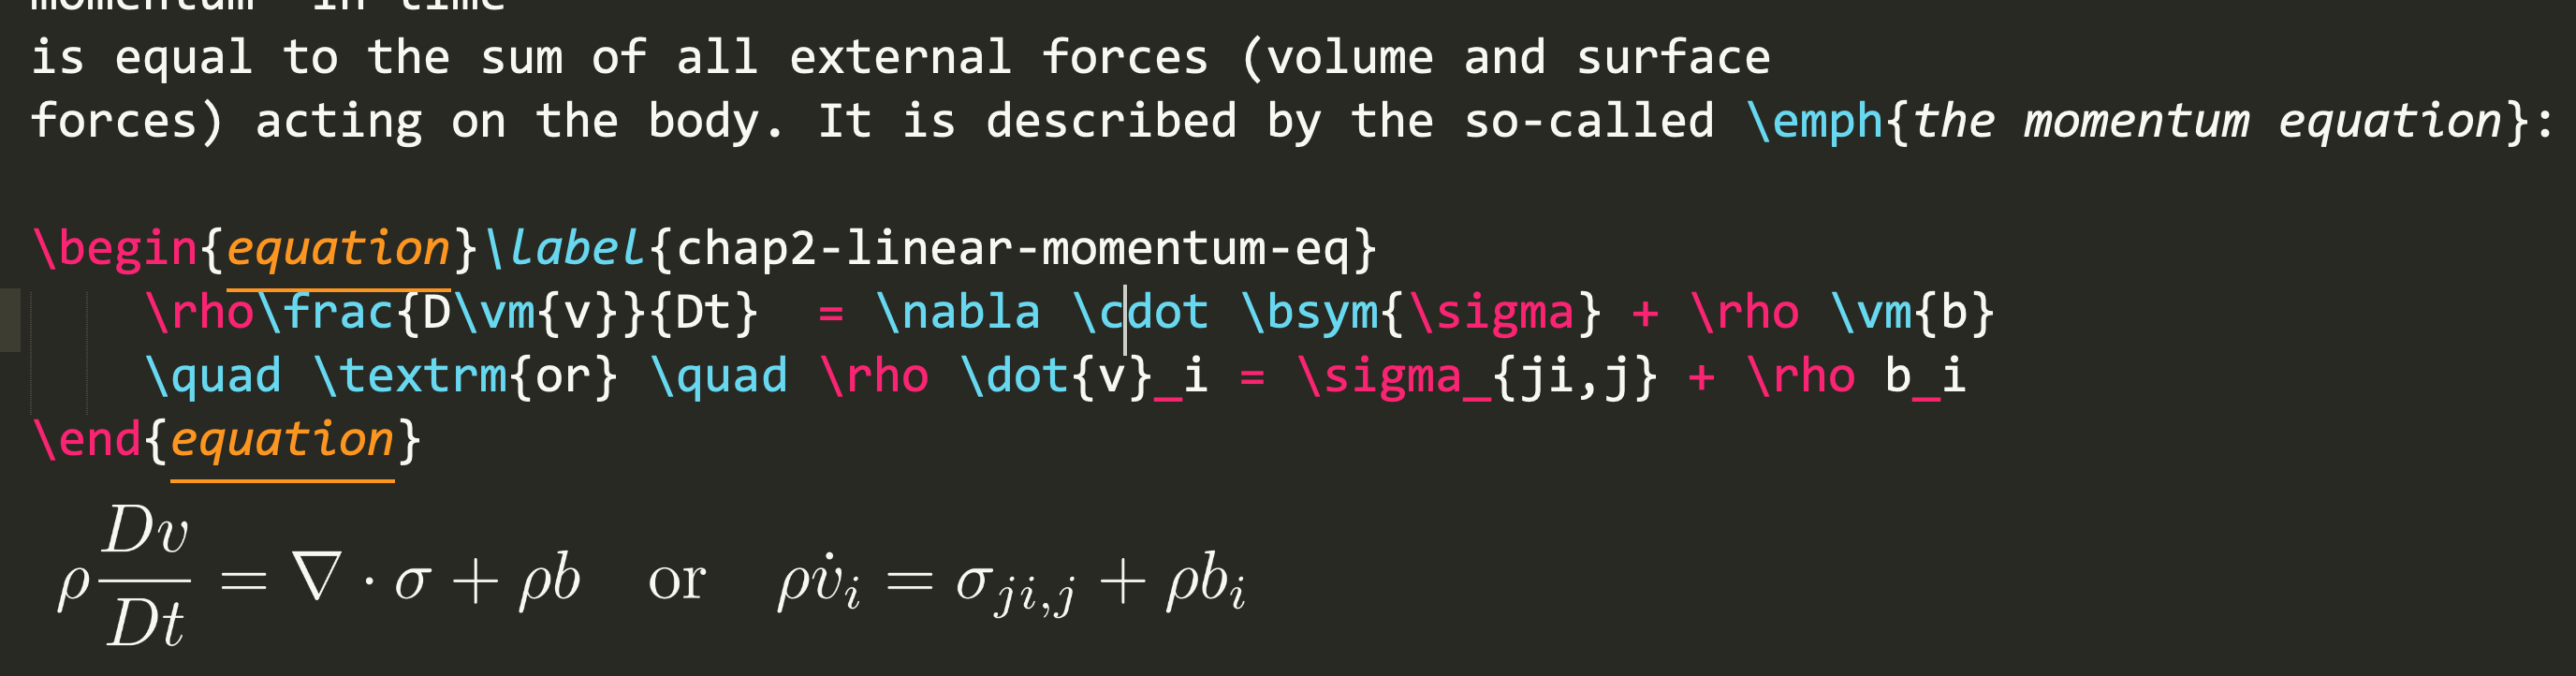
\includegraphics[width=0.65\textwidth]{sublime-text}
   \caption{\texttt{Sublime Text} can render equations in real time.}
\label{fig:sublime-text}
\end{figure}
\end{rmk}


%%%%%%%%%%%%%%%%%%%%%%%%%%%%%%%
\section{Writing tips}\label{sec:writing-tips}

\cref{sec:guidelines}
\cref{sec:writing-process}
\cref{structure}
\cref{sec:mistakes}

\url{https://www.youtube.com/watch?v=VK51E3gHENc}.

%--------------------------------------
\subsection{General guidelines}\label{sec:guidelines}

The following general guidelines are nothing new but they are worthy repeated:

\begin{enumerate}
\item To inform not to impress;
\item Aims for clarity and readability;
\item Contributions must be clearly stated;
\item Each paragraph conveys only a single idea or message;
\item Avoid jargon;%  Writing a paper is not a race for complexity. You should make it as simple as possible for a neophyte reader to understand;
\item Aims for reproducibility;
\item Try to minimize the chances for reviewers to raise issues;
\end{enumerate}

The main contributions of the paper must be clearly stated after a brief review of the literature. How your work differs from the existing literature in such and such a way. Be precise, this is where the reviewers will try to find problems with your work. Their goal is to identify whether your work is novel. If it is not immediately clear from the Abstract and Introduction you risk being unconvincing. 

Do not be afraid of writing short paragraphs, even two-sentence ones. Each paragraph conveys only a single idea or message.


Avoid jargon.  Writing a paper is not a race for complexity. You should make it as simple as possible for a neophyte reader to understand;

Reproducibility is a big issue in scientific research nowadays. However, we just confine to the situation where a published simulation result is genuinely correct but impossible to reproduce by people rather than the authors. The world would be a better place if all the authors are more thoughtful when reporting their results: all information needed to make that particular simulation work should be provided. Particularly, nontrivial parameters.

You can save time for both you -- the authors -- and the reviewers by not making them guess. For example, if you do not do large deformation simulations, make it clear and justify that choice. If you have used a particular value for one numerical parameter, explain your choice.

%--------------------------------------
\subsection{Writing process: an iterative process}\label{sec:writing-process}

The first idea is when you have finished your last simulation, the first draft of your full paper is complete. Here by you we mean the co-author of the paper who is in charge of the writing. After that, it is just polishing the paper. The second idea is to not lose motivation due to set backs. That is, if the simulations are not working, don't be upset; let's write something instead. It can be filling Section \textit{Acknowledgments}. Having updated your paper definitely makes us feel good. And that is very important. 


After a research idea has been developed, one should start writing the paper. Obviously, the paper is empty, see \cref{snippet_template} for a \LaTeX\ file for an empty paper.
%---------------------------------------------------------------------------
\begin{figure*}[!h]
  \begin{snippetlatex}[caption={Input file for the plate penetration problem.},label={snippet_template},framerule=1pt,tabsize=3]
    \documentclass[authoryear,3p,times,preprint,review,fleqn]{elsarticle}
    \title{\textbf{}}
    \begin{abstract}
    \end{abstract}
    \section{Introduction}
    \section{Methodology}
    \section{Examples}
    \section*{Acknowledgments}
    \bibliographystyle{abbrvnat} % => just V. P. Nguyen, not Phu Nguyen, ...
    \bibliography{mpm}
  \end{snippetlatex}
\end{figure*}
%---------------------------------------------------------------------------

For the sake of presentation, let's assume that one needs to develop a formulation, implement it in a code, and carry out simulations using this code. Then, one first works on the formulation. When there is some progresses, one can write some key equations in the paper (filling Section \textit{Methodology}). Having the formulations nicely written in a pdf can help you to spot errors. Now that the formulation has been complete, one moves to the implementation. Again, this task should be intertwined  with the writing as well (filling Section \textit{Methodology}). Most often, one starts with a very simple problem to test the code (and the idea). If this example works, one is confident about the idea, he/she can write something on Section \textit{Introduction} while the second simulation is under way. If this example is important, she can write about it in Section \textit{Examples}. If she is lucky, the result of this second simulation is very good. She can now fill  Sections \textit{Introduction} and  \textit{Abstract} while working on the third simulation.

If you feel stuck at writing any parts of the paper, feel free to do something else because keep focusing on the writing does not always help. Most often ideas come when you are in a diffuse mode, a concept proposed in \cite{Oakley:2018a}. For example, while playing with your kids on a playground, the idea for writing a good abstract usually comes. Jotting down the idea on a phone and you're done with this part of the paper.

While working on this paper, we read the literature (we always read it anyway). If we find a good paper relevant to our work, put it in \texttt{Bibdesk}, and cite it in the paper with some key sentences about it. Doing so saves us a lot of time by not re-discovering this paper in the future. Note that \texttt{Bibdesk} can link a pdf to a paper. Therefore, we can have a library of papers on top of a bib file. 


%%%%%%%%%%%%%%%%%%%%%%%%%%%%%%%
\subsection{How to structure your paper}\label{structure}

An excellent article on how to structure a scientific paper can be found at \url{https://www.nature.com/scitable/topicpage/scientific-papers-13815490/}. We will not repeat that herein. Instead, we elaborate some of the arguments such as a complex section should have a global paragraph before going into its subsection, what the conclusion section should include.  

\begin{figure}[!h]
  \centering
  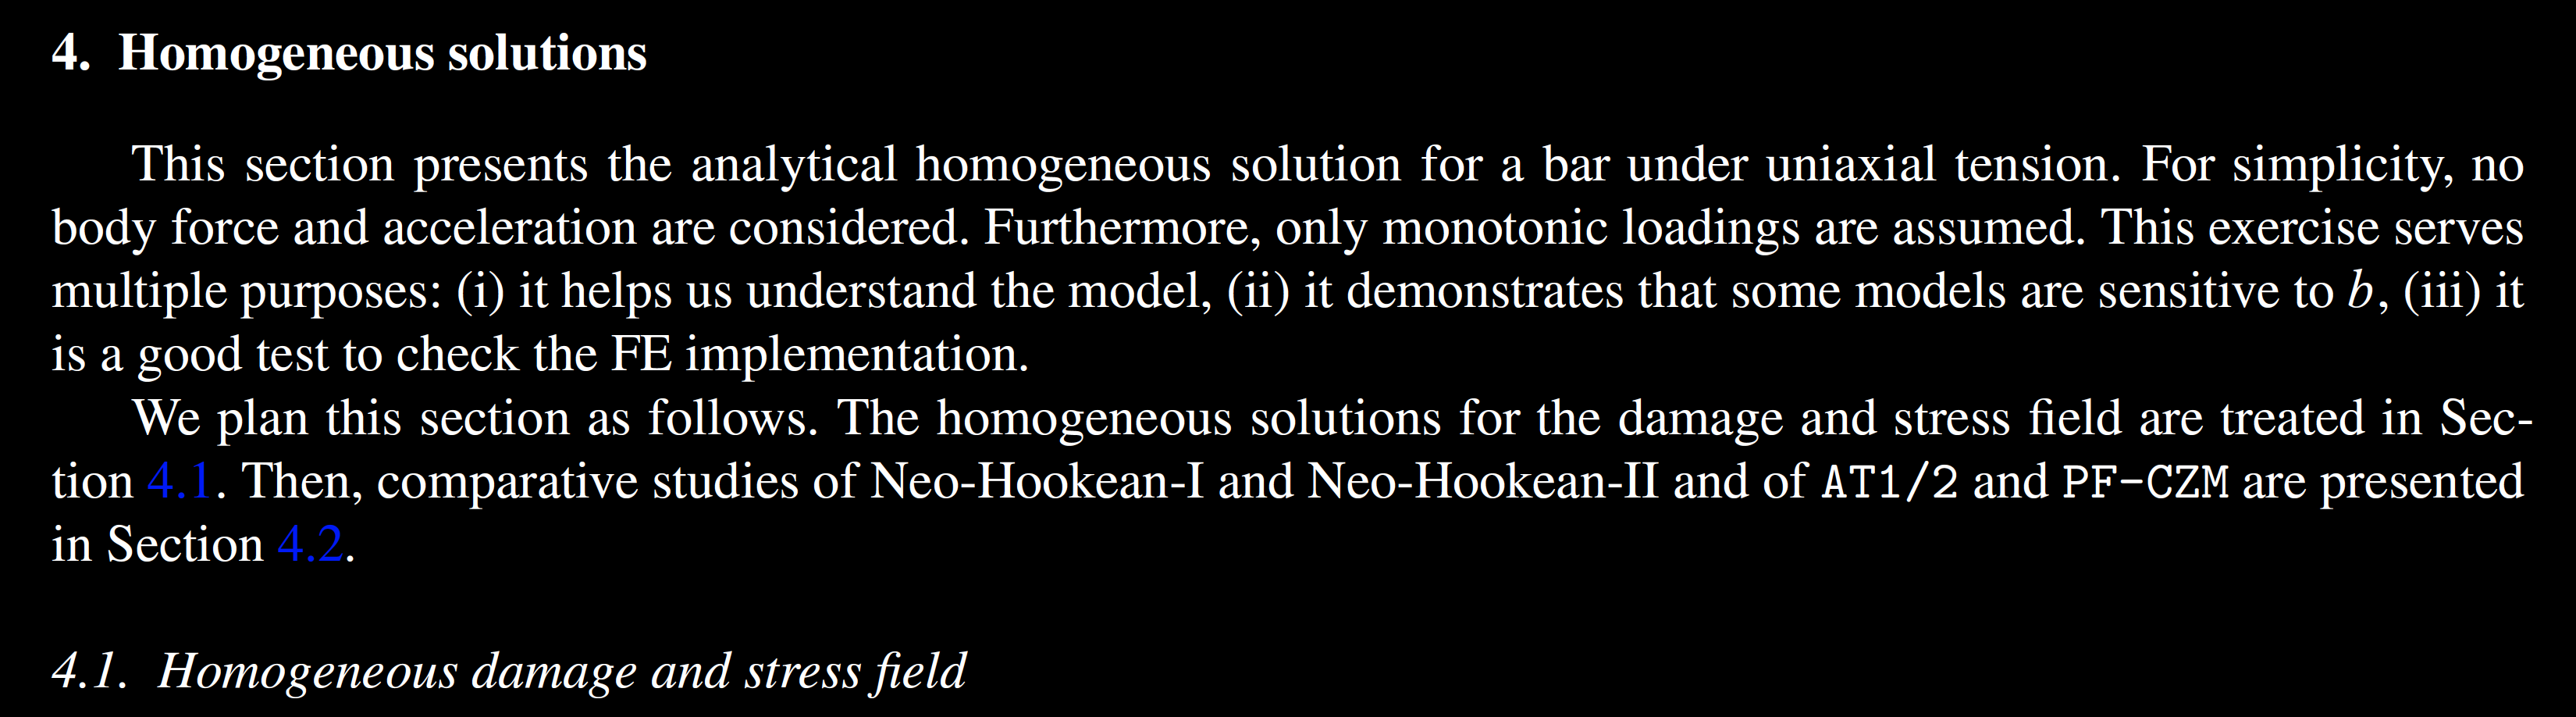
\includegraphics[width=0.9\textwidth]{section}
  \caption{A complex section should have a global paragraph between the heading of a section and the heading of its first subsection.}
  \label{fig:section}
\end{figure}

For paragraphs that are quite complex it is a good idea to write a global paragraph between the heading of a section and the heading of its first subsection. See \cref{fig:section} for an example. remember to prepare your readers for the structure ahead at all levels. 

Papers on the field of computational engineering and sciences always have a section, typically named `Numerical Examples' where some tests are presented to demonstrate the performance of the model/theory presented. While these examples are most often presented in order of increasing complexity, we can do a better job in presenting them. For example, a global paragraph stating why these examples were chosen, which open source (if it is the case) code was used etc.

There are two misunderstandings about the Conclusion section. First, the Conclusion section is made long under the false belief that a longer Conclusion will seem more impressive.

% 
%--------------------------------------
\subsection{Some common mistakes}\label{sec:mistakes}

\cref{tab:mistakes}.

%%%%%%%%%%%%%%%%%%%%%%%%%%%%%%%%%%%%%%%%%%%%%%%%%%
\setlength{\fboxsep}{0pt}
\begin{table}[h!]
   \centering
     \setlength\fboxsep{0pt}
\vskip-\topsep%
\smallskip%
%\renewcommand\arraystretch{1.3}
\colorbox{darkgray}{%
   \begin{tabularx}{0.7\textwidth}{ll}
   \toprule
   Don't & Do  \\
  \midrule
  The Table/Figure 2 & Table/Figure 2 \\
  The Equation (2.2) & Equation (2.2) \\
  \bottomrule
 \end{tabularx}%
 }
\caption{Some common mistakes.}
 \label{tab:mistakes}
\end{table}


%%%%%%%%%%%%%%%%%%%%%%%%%%%%%%%
\section{\LaTeX\ tips}\label{sec:latex}

To improve the writing experience, once in while one should update their \LaTeX\ skills. \cref{snippet_latex_packages} provides an updated list of \LaTeX\ packages being used to write our papers.
By setting the option \textit{backref=page} for the package \texttt{hyperref}, there appears `Cited on page \#' at the end of all references. 

Using standard cross-referencing in \LaTeX\ only produces the label number, a name describing the label such as figure, chapter or equation has to be added manually. The cleveref package overcomes this limitation by automatically producing the label name and number:

\begin{verbatim}
\cref{fig:figure1}, instead of Fig.~\ref{fig:figure1}
\cref{eq:equation1}, instead of Eq.~\ref{eq:equation1}
\end{verbatim}

%---------------------------------------------------------------------------
\begin{figure*}[!h]
  \begin{snippetlatex}[caption={Commonly used \LaTeX\ packages.},label={snippet_latex_packages},framerule=1pt,tabsize=3]
    \usepackage{amsmath,amssymb, mathtools,mathrsfs,stmaryrd,titletoc}
    \usepackage{natbib}
    \usepackage[scaled=0.92]{helvet}  % set Helvetica as the sans-serif font
    \renewcommand{\rmdefault}{ptm}    % set Times as the default text font
    \usepackage[retainorgcmds]{IEEEtrantools}
    \usepackage[usenames]{color}
    \usepackage{tabularx}
    \usepackage{booktabs}    
    \usepackage[font=small,labelfont=md]{caption,subfig}
    \usepackage{multirow}
    \usepackage[T1]{fontenc} % typing french                        
    \usepackage[bookmarks=true,colorlinks=true,linkcolor=blue,backref=page]{hyperref}
    \usepackage{float}         % make new float environment such as boxes (captioned)
    \usepackage{listings}      % insert source code   
    \usepackage{algorithm}
    \usepackage{algorithmicx}
    \usepackage{algpseudocode}
    \usepackage[activate={true,nocompatibility},final,tracking=true,
    kerning=true,spacing=true,factor=1100,stretch=10,shrink=10]{microtype}
    \usepackage[capitalise]{cleveref} %Basically, cleveref must be loaded last.

    \definecolor{darkgray}{rgb}{0.95,0.95,0.95} % color used in tables
    % cleverref package: just do \cref{label} for figures, tables, equations anything
    % the package will determine the correct prefix be it Fig. or Equation or Listing.
    \crefname{figure}{Fig.}{Figs.}  
    \crefname{equation}{Equation}{Equations}

    \renewcommand*{\backref}[1]{}
    \renewcommand*{\backrefalt}[4]{[{%
        \ifcase #1 %
              \or Cited on page~#2%
              \else Cited on pages #2%
        \fi%
        }]}
  \end{snippetlatex}
\end{figure*}
%---------------------------------------------------------------------------

In what follows, we discuss how to prepare high quality plots in \cref{sec:figs}, tables in 
\cref{sec:tabs}. \cref{sec:equation}

%%%%%%%%%%%%%%%%%%%%%%
\subsection{Figures}\label{sec:figs}

It is not a requirement that the font used in figures match that of the text. Yet, it would be better if they match. \cref{fig:cold-spray-plot} is such a figure. And the \LaTeX\ code is shown in \cref{snippet_latex_figure}. This \texttt{Matplotlib} based \texttt{Python} script, given in \cref{snippet_matplotlib}, produces a PDF image with font not exactly matching the text font. If you really want the font in your plots exactly match that in the text, see \cref{fig:cold-spray-plot-pgf} for such an example, the script in \cref{snippet_matplotlib_pgf} can be used.

%---------------------------------------------------------------------------
\begin{figure*}[!h]
  \begin{snippetlatex}[caption={Input file for the plate penetration problem.},label={snippet_latex_figure},framerule=1pt,tabsize=3]
    \begin{figure}[!ht]
      \centering
      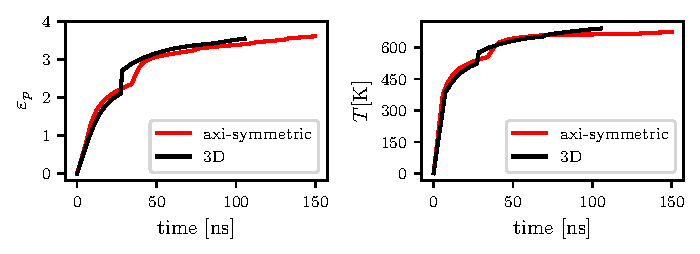
\includegraphics{cold-spray-plots.pfd} # insert a PDF
      %% Creator: Matplotlib, PGF backend
%%
%% To include the figure in your LaTeX document, write
%%   \input{<filename>.pgf}
%%
%% Make sure the required packages are loaded in your preamble
%%   \usepackage{pgf}
%%
%% Figures using additional raster images can only be included by \input if
%% they are in the same directory as the main LaTeX file. For loading figures
%% from other directories you can use the `import` package
%%   \usepackage{import}
%% and then include the figures with
%%   \import{<path to file>}{<filename>.pgf}
%%
%% Matplotlib used the following preamble
%%   \usepackage[utf8x]{inputenc}
%%   \usepackage[T1]{fontenc}
%%   \newcommand{\vect}[1]{#1}
%%
\begingroup%
\makeatletter%
\begin{pgfpicture}%
\pgfpathrectangle{\pgfpointorigin}{\pgfqpoint{6.375716in}{2.328394in}}%
\pgfusepath{use as bounding box, clip}%
\begin{pgfscope}%
\pgfsetbuttcap%
\pgfsetmiterjoin%
\definecolor{currentfill}{rgb}{1.000000,1.000000,1.000000}%
\pgfsetfillcolor{currentfill}%
\pgfsetlinewidth{0.000000pt}%
\definecolor{currentstroke}{rgb}{1.000000,1.000000,1.000000}%
\pgfsetstrokecolor{currentstroke}%
\pgfsetdash{}{0pt}%
\pgfpathmoveto{\pgfqpoint{0.000000in}{0.000000in}}%
\pgfpathlineto{\pgfqpoint{6.375716in}{0.000000in}}%
\pgfpathlineto{\pgfqpoint{6.375716in}{2.328394in}}%
\pgfpathlineto{\pgfqpoint{0.000000in}{2.328394in}}%
\pgfpathclose%
\pgfusepath{fill}%
\end{pgfscope}%
\begin{pgfscope}%
\pgfsetbuttcap%
\pgfsetmiterjoin%
\definecolor{currentfill}{rgb}{1.000000,1.000000,1.000000}%
\pgfsetfillcolor{currentfill}%
\pgfsetlinewidth{0.000000pt}%
\definecolor{currentstroke}{rgb}{0.000000,0.000000,0.000000}%
\pgfsetstrokecolor{currentstroke}%
\pgfsetstrokeopacity{0.000000}%
\pgfsetdash{}{0pt}%
\pgfpathmoveto{\pgfqpoint{0.434462in}{0.489757in}}%
\pgfpathlineto{\pgfqpoint{3.045729in}{0.489757in}}%
\pgfpathlineto{\pgfqpoint{3.045729in}{2.190131in}}%
\pgfpathlineto{\pgfqpoint{0.434462in}{2.190131in}}%
\pgfpathclose%
\pgfusepath{fill}%
\end{pgfscope}%
\begin{pgfscope}%
\pgfsetbuttcap%
\pgfsetroundjoin%
\definecolor{currentfill}{rgb}{0.000000,0.000000,0.000000}%
\pgfsetfillcolor{currentfill}%
\pgfsetlinewidth{0.803000pt}%
\definecolor{currentstroke}{rgb}{0.000000,0.000000,0.000000}%
\pgfsetstrokecolor{currentstroke}%
\pgfsetdash{}{0pt}%
\pgfsys@defobject{currentmarker}{\pgfqpoint{0.000000in}{-0.048611in}}{\pgfqpoint{0.000000in}{0.000000in}}{%
\pgfpathmoveto{\pgfqpoint{0.000000in}{0.000000in}}%
\pgfpathlineto{\pgfqpoint{0.000000in}{-0.048611in}}%
\pgfusepath{stroke,fill}%
}%
\begin{pgfscope}%
\pgfsys@transformshift{0.553156in}{0.489757in}%
\pgfsys@useobject{currentmarker}{}%
\end{pgfscope}%
\end{pgfscope}%
\begin{pgfscope}%
\definecolor{textcolor}{rgb}{0.000000,0.000000,0.000000}%
\pgfsetstrokecolor{textcolor}%
\pgfsetfillcolor{textcolor}%
\pgftext[x=0.553156in,y=0.392535in,,top]{\color{textcolor}\rmfamily\fontsize{8.000000}{9.600000}\selectfont \(\displaystyle 0\)}%
\end{pgfscope}%
\begin{pgfscope}%
\pgfsetbuttcap%
\pgfsetroundjoin%
\definecolor{currentfill}{rgb}{0.000000,0.000000,0.000000}%
\pgfsetfillcolor{currentfill}%
\pgfsetlinewidth{0.803000pt}%
\definecolor{currentstroke}{rgb}{0.000000,0.000000,0.000000}%
\pgfsetstrokecolor{currentstroke}%
\pgfsetdash{}{0pt}%
\pgfsys@defobject{currentmarker}{\pgfqpoint{0.000000in}{-0.048611in}}{\pgfqpoint{0.000000in}{0.000000in}}{%
\pgfpathmoveto{\pgfqpoint{0.000000in}{0.000000in}}%
\pgfpathlineto{\pgfqpoint{0.000000in}{-0.048611in}}%
\pgfusepath{stroke,fill}%
}%
\begin{pgfscope}%
\pgfsys@transformshift{0.948881in}{0.489757in}%
\pgfsys@useobject{currentmarker}{}%
\end{pgfscope}%
\end{pgfscope}%
\begin{pgfscope}%
\definecolor{textcolor}{rgb}{0.000000,0.000000,0.000000}%
\pgfsetstrokecolor{textcolor}%
\pgfsetfillcolor{textcolor}%
\pgftext[x=0.948881in,y=0.392535in,,top]{\color{textcolor}\rmfamily\fontsize{8.000000}{9.600000}\selectfont \(\displaystyle 25\)}%
\end{pgfscope}%
\begin{pgfscope}%
\pgfsetbuttcap%
\pgfsetroundjoin%
\definecolor{currentfill}{rgb}{0.000000,0.000000,0.000000}%
\pgfsetfillcolor{currentfill}%
\pgfsetlinewidth{0.803000pt}%
\definecolor{currentstroke}{rgb}{0.000000,0.000000,0.000000}%
\pgfsetstrokecolor{currentstroke}%
\pgfsetdash{}{0pt}%
\pgfsys@defobject{currentmarker}{\pgfqpoint{0.000000in}{-0.048611in}}{\pgfqpoint{0.000000in}{0.000000in}}{%
\pgfpathmoveto{\pgfqpoint{0.000000in}{0.000000in}}%
\pgfpathlineto{\pgfqpoint{0.000000in}{-0.048611in}}%
\pgfusepath{stroke,fill}%
}%
\begin{pgfscope}%
\pgfsys@transformshift{1.344607in}{0.489757in}%
\pgfsys@useobject{currentmarker}{}%
\end{pgfscope}%
\end{pgfscope}%
\begin{pgfscope}%
\definecolor{textcolor}{rgb}{0.000000,0.000000,0.000000}%
\pgfsetstrokecolor{textcolor}%
\pgfsetfillcolor{textcolor}%
\pgftext[x=1.344607in,y=0.392535in,,top]{\color{textcolor}\rmfamily\fontsize{8.000000}{9.600000}\selectfont \(\displaystyle 50\)}%
\end{pgfscope}%
\begin{pgfscope}%
\pgfsetbuttcap%
\pgfsetroundjoin%
\definecolor{currentfill}{rgb}{0.000000,0.000000,0.000000}%
\pgfsetfillcolor{currentfill}%
\pgfsetlinewidth{0.803000pt}%
\definecolor{currentstroke}{rgb}{0.000000,0.000000,0.000000}%
\pgfsetstrokecolor{currentstroke}%
\pgfsetdash{}{0pt}%
\pgfsys@defobject{currentmarker}{\pgfqpoint{0.000000in}{-0.048611in}}{\pgfqpoint{0.000000in}{0.000000in}}{%
\pgfpathmoveto{\pgfqpoint{0.000000in}{0.000000in}}%
\pgfpathlineto{\pgfqpoint{0.000000in}{-0.048611in}}%
\pgfusepath{stroke,fill}%
}%
\begin{pgfscope}%
\pgfsys@transformshift{1.740333in}{0.489757in}%
\pgfsys@useobject{currentmarker}{}%
\end{pgfscope}%
\end{pgfscope}%
\begin{pgfscope}%
\definecolor{textcolor}{rgb}{0.000000,0.000000,0.000000}%
\pgfsetstrokecolor{textcolor}%
\pgfsetfillcolor{textcolor}%
\pgftext[x=1.740333in,y=0.392535in,,top]{\color{textcolor}\rmfamily\fontsize{8.000000}{9.600000}\selectfont \(\displaystyle 75\)}%
\end{pgfscope}%
\begin{pgfscope}%
\pgfsetbuttcap%
\pgfsetroundjoin%
\definecolor{currentfill}{rgb}{0.000000,0.000000,0.000000}%
\pgfsetfillcolor{currentfill}%
\pgfsetlinewidth{0.803000pt}%
\definecolor{currentstroke}{rgb}{0.000000,0.000000,0.000000}%
\pgfsetstrokecolor{currentstroke}%
\pgfsetdash{}{0pt}%
\pgfsys@defobject{currentmarker}{\pgfqpoint{0.000000in}{-0.048611in}}{\pgfqpoint{0.000000in}{0.000000in}}{%
\pgfpathmoveto{\pgfqpoint{0.000000in}{0.000000in}}%
\pgfpathlineto{\pgfqpoint{0.000000in}{-0.048611in}}%
\pgfusepath{stroke,fill}%
}%
\begin{pgfscope}%
\pgfsys@transformshift{2.136059in}{0.489757in}%
\pgfsys@useobject{currentmarker}{}%
\end{pgfscope}%
\end{pgfscope}%
\begin{pgfscope}%
\definecolor{textcolor}{rgb}{0.000000,0.000000,0.000000}%
\pgfsetstrokecolor{textcolor}%
\pgfsetfillcolor{textcolor}%
\pgftext[x=2.136059in,y=0.392535in,,top]{\color{textcolor}\rmfamily\fontsize{8.000000}{9.600000}\selectfont \(\displaystyle 100\)}%
\end{pgfscope}%
\begin{pgfscope}%
\pgfsetbuttcap%
\pgfsetroundjoin%
\definecolor{currentfill}{rgb}{0.000000,0.000000,0.000000}%
\pgfsetfillcolor{currentfill}%
\pgfsetlinewidth{0.803000pt}%
\definecolor{currentstroke}{rgb}{0.000000,0.000000,0.000000}%
\pgfsetstrokecolor{currentstroke}%
\pgfsetdash{}{0pt}%
\pgfsys@defobject{currentmarker}{\pgfqpoint{0.000000in}{-0.048611in}}{\pgfqpoint{0.000000in}{0.000000in}}{%
\pgfpathmoveto{\pgfqpoint{0.000000in}{0.000000in}}%
\pgfpathlineto{\pgfqpoint{0.000000in}{-0.048611in}}%
\pgfusepath{stroke,fill}%
}%
\begin{pgfscope}%
\pgfsys@transformshift{2.531785in}{0.489757in}%
\pgfsys@useobject{currentmarker}{}%
\end{pgfscope}%
\end{pgfscope}%
\begin{pgfscope}%
\definecolor{textcolor}{rgb}{0.000000,0.000000,0.000000}%
\pgfsetstrokecolor{textcolor}%
\pgfsetfillcolor{textcolor}%
\pgftext[x=2.531785in,y=0.392535in,,top]{\color{textcolor}\rmfamily\fontsize{8.000000}{9.600000}\selectfont \(\displaystyle 125\)}%
\end{pgfscope}%
\begin{pgfscope}%
\pgfsetbuttcap%
\pgfsetroundjoin%
\definecolor{currentfill}{rgb}{0.000000,0.000000,0.000000}%
\pgfsetfillcolor{currentfill}%
\pgfsetlinewidth{0.803000pt}%
\definecolor{currentstroke}{rgb}{0.000000,0.000000,0.000000}%
\pgfsetstrokecolor{currentstroke}%
\pgfsetdash{}{0pt}%
\pgfsys@defobject{currentmarker}{\pgfqpoint{0.000000in}{-0.048611in}}{\pgfqpoint{0.000000in}{0.000000in}}{%
\pgfpathmoveto{\pgfqpoint{0.000000in}{0.000000in}}%
\pgfpathlineto{\pgfqpoint{0.000000in}{-0.048611in}}%
\pgfusepath{stroke,fill}%
}%
\begin{pgfscope}%
\pgfsys@transformshift{2.927510in}{0.489757in}%
\pgfsys@useobject{currentmarker}{}%
\end{pgfscope}%
\end{pgfscope}%
\begin{pgfscope}%
\definecolor{textcolor}{rgb}{0.000000,0.000000,0.000000}%
\pgfsetstrokecolor{textcolor}%
\pgfsetfillcolor{textcolor}%
\pgftext[x=2.927510in,y=0.392535in,,top]{\color{textcolor}\rmfamily\fontsize{8.000000}{9.600000}\selectfont \(\displaystyle 150\)}%
\end{pgfscope}%
\begin{pgfscope}%
\definecolor{textcolor}{rgb}{0.000000,0.000000,0.000000}%
\pgfsetstrokecolor{textcolor}%
\pgfsetfillcolor{textcolor}%
\pgftext[x=1.740096in,y=0.238855in,,top]{\color{textcolor}\rmfamily\fontsize{10.000000}{12.000000}\selectfont time [ns]}%
\end{pgfscope}%
\begin{pgfscope}%
\pgfsetbuttcap%
\pgfsetroundjoin%
\definecolor{currentfill}{rgb}{0.000000,0.000000,0.000000}%
\pgfsetfillcolor{currentfill}%
\pgfsetlinewidth{0.803000pt}%
\definecolor{currentstroke}{rgb}{0.000000,0.000000,0.000000}%
\pgfsetstrokecolor{currentstroke}%
\pgfsetdash{}{0pt}%
\pgfsys@defobject{currentmarker}{\pgfqpoint{-0.048611in}{0.000000in}}{\pgfqpoint{0.000000in}{0.000000in}}{%
\pgfpathmoveto{\pgfqpoint{0.000000in}{0.000000in}}%
\pgfpathlineto{\pgfqpoint{-0.048611in}{0.000000in}}%
\pgfusepath{stroke,fill}%
}%
\begin{pgfscope}%
\pgfsys@transformshift{0.434462in}{0.563078in}%
\pgfsys@useobject{currentmarker}{}%
\end{pgfscope}%
\end{pgfscope}%
\begin{pgfscope}%
\definecolor{textcolor}{rgb}{0.000000,0.000000,0.000000}%
\pgfsetstrokecolor{textcolor}%
\pgfsetfillcolor{textcolor}%
\pgftext[x=0.278211in,y=0.524816in,left,base]{\color{textcolor}\rmfamily\fontsize{8.000000}{9.600000}\selectfont \(\displaystyle 0\)}%
\end{pgfscope}%
\begin{pgfscope}%
\pgfsetbuttcap%
\pgfsetroundjoin%
\definecolor{currentfill}{rgb}{0.000000,0.000000,0.000000}%
\pgfsetfillcolor{currentfill}%
\pgfsetlinewidth{0.803000pt}%
\definecolor{currentstroke}{rgb}{0.000000,0.000000,0.000000}%
\pgfsetstrokecolor{currentstroke}%
\pgfsetdash{}{0pt}%
\pgfsys@defobject{currentmarker}{\pgfqpoint{-0.048611in}{0.000000in}}{\pgfqpoint{0.000000in}{0.000000in}}{%
\pgfpathmoveto{\pgfqpoint{0.000000in}{0.000000in}}%
\pgfpathlineto{\pgfqpoint{-0.048611in}{0.000000in}}%
\pgfusepath{stroke,fill}%
}%
\begin{pgfscope}%
\pgfsys@transformshift{0.434462in}{0.969841in}%
\pgfsys@useobject{currentmarker}{}%
\end{pgfscope}%
\end{pgfscope}%
\begin{pgfscope}%
\definecolor{textcolor}{rgb}{0.000000,0.000000,0.000000}%
\pgfsetstrokecolor{textcolor}%
\pgfsetfillcolor{textcolor}%
\pgftext[x=0.278211in,y=0.931579in,left,base]{\color{textcolor}\rmfamily\fontsize{8.000000}{9.600000}\selectfont \(\displaystyle 1\)}%
\end{pgfscope}%
\begin{pgfscope}%
\pgfsetbuttcap%
\pgfsetroundjoin%
\definecolor{currentfill}{rgb}{0.000000,0.000000,0.000000}%
\pgfsetfillcolor{currentfill}%
\pgfsetlinewidth{0.803000pt}%
\definecolor{currentstroke}{rgb}{0.000000,0.000000,0.000000}%
\pgfsetstrokecolor{currentstroke}%
\pgfsetdash{}{0pt}%
\pgfsys@defobject{currentmarker}{\pgfqpoint{-0.048611in}{0.000000in}}{\pgfqpoint{0.000000in}{0.000000in}}{%
\pgfpathmoveto{\pgfqpoint{0.000000in}{0.000000in}}%
\pgfpathlineto{\pgfqpoint{-0.048611in}{0.000000in}}%
\pgfusepath{stroke,fill}%
}%
\begin{pgfscope}%
\pgfsys@transformshift{0.434462in}{1.376605in}%
\pgfsys@useobject{currentmarker}{}%
\end{pgfscope}%
\end{pgfscope}%
\begin{pgfscope}%
\definecolor{textcolor}{rgb}{0.000000,0.000000,0.000000}%
\pgfsetstrokecolor{textcolor}%
\pgfsetfillcolor{textcolor}%
\pgftext[x=0.278211in,y=1.338342in,left,base]{\color{textcolor}\rmfamily\fontsize{8.000000}{9.600000}\selectfont \(\displaystyle 2\)}%
\end{pgfscope}%
\begin{pgfscope}%
\pgfsetbuttcap%
\pgfsetroundjoin%
\definecolor{currentfill}{rgb}{0.000000,0.000000,0.000000}%
\pgfsetfillcolor{currentfill}%
\pgfsetlinewidth{0.803000pt}%
\definecolor{currentstroke}{rgb}{0.000000,0.000000,0.000000}%
\pgfsetstrokecolor{currentstroke}%
\pgfsetdash{}{0pt}%
\pgfsys@defobject{currentmarker}{\pgfqpoint{-0.048611in}{0.000000in}}{\pgfqpoint{0.000000in}{0.000000in}}{%
\pgfpathmoveto{\pgfqpoint{0.000000in}{0.000000in}}%
\pgfpathlineto{\pgfqpoint{-0.048611in}{0.000000in}}%
\pgfusepath{stroke,fill}%
}%
\begin{pgfscope}%
\pgfsys@transformshift{0.434462in}{1.783368in}%
\pgfsys@useobject{currentmarker}{}%
\end{pgfscope}%
\end{pgfscope}%
\begin{pgfscope}%
\definecolor{textcolor}{rgb}{0.000000,0.000000,0.000000}%
\pgfsetstrokecolor{textcolor}%
\pgfsetfillcolor{textcolor}%
\pgftext[x=0.278211in,y=1.745106in,left,base]{\color{textcolor}\rmfamily\fontsize{8.000000}{9.600000}\selectfont \(\displaystyle 3\)}%
\end{pgfscope}%
\begin{pgfscope}%
\pgfsetbuttcap%
\pgfsetroundjoin%
\definecolor{currentfill}{rgb}{0.000000,0.000000,0.000000}%
\pgfsetfillcolor{currentfill}%
\pgfsetlinewidth{0.803000pt}%
\definecolor{currentstroke}{rgb}{0.000000,0.000000,0.000000}%
\pgfsetstrokecolor{currentstroke}%
\pgfsetdash{}{0pt}%
\pgfsys@defobject{currentmarker}{\pgfqpoint{-0.048611in}{0.000000in}}{\pgfqpoint{0.000000in}{0.000000in}}{%
\pgfpathmoveto{\pgfqpoint{0.000000in}{0.000000in}}%
\pgfpathlineto{\pgfqpoint{-0.048611in}{0.000000in}}%
\pgfusepath{stroke,fill}%
}%
\begin{pgfscope}%
\pgfsys@transformshift{0.434462in}{2.190131in}%
\pgfsys@useobject{currentmarker}{}%
\end{pgfscope}%
\end{pgfscope}%
\begin{pgfscope}%
\definecolor{textcolor}{rgb}{0.000000,0.000000,0.000000}%
\pgfsetstrokecolor{textcolor}%
\pgfsetfillcolor{textcolor}%
\pgftext[x=0.278211in,y=2.151869in,left,base]{\color{textcolor}\rmfamily\fontsize{8.000000}{9.600000}\selectfont \(\displaystyle 4\)}%
\end{pgfscope}%
\begin{pgfscope}%
\definecolor{textcolor}{rgb}{0.000000,0.000000,0.000000}%
\pgfsetstrokecolor{textcolor}%
\pgfsetfillcolor{textcolor}%
\pgftext[x=0.222655in,y=1.339944in,,bottom,rotate=90.000000]{\color{textcolor}\rmfamily\fontsize{10.000000}{12.000000}\selectfont \(\displaystyle \varepsilon_p\)}%
\end{pgfscope}%
\begin{pgfscope}%
\pgfpathrectangle{\pgfqpoint{0.434462in}{0.489757in}}{\pgfqpoint{2.611268in}{1.700374in}}%
\pgfusepath{clip}%
\pgfsetrectcap%
\pgfsetroundjoin%
\pgfsetlinewidth{1.505625pt}%
\definecolor{currentstroke}{rgb}{1.000000,0.000000,0.000000}%
\pgfsetstrokecolor{currentstroke}%
\pgfsetdash{}{0pt}%
\pgfpathmoveto{\pgfqpoint{0.553156in}{0.563078in}}%
\pgfpathlineto{\pgfqpoint{0.644136in}{0.898446in}}%
\pgfpathlineto{\pgfqpoint{0.677856in}{1.049453in}}%
\pgfpathlineto{\pgfqpoint{0.701275in}{1.128621in}}%
\pgfpathlineto{\pgfqpoint{0.720070in}{1.178198in}}%
\pgfpathlineto{\pgfqpoint{0.750463in}{1.247038in}}%
\pgfpathlineto{\pgfqpoint{0.763527in}{1.269512in}}%
\pgfpathlineto{\pgfqpoint{0.787471in}{1.301349in}}%
\pgfpathlineto{\pgfqpoint{0.819226in}{1.343112in}}%
\pgfpathlineto{\pgfqpoint{0.838567in}{1.361445in}}%
\pgfpathlineto{\pgfqpoint{0.899727in}{1.413807in}}%
\pgfpathlineto{\pgfqpoint{0.923829in}{1.429057in}}%
\pgfpathlineto{\pgfqpoint{0.946966in}{1.443696in}}%
\pgfpathlineto{\pgfqpoint{0.961875in}{1.454223in}}%
\pgfpathlineto{\pgfqpoint{0.983819in}{1.465991in}}%
\pgfpathlineto{\pgfqpoint{1.019222in}{1.483819in}}%
\pgfpathlineto{\pgfqpoint{1.032951in}{1.491572in}}%
\pgfpathlineto{\pgfqpoint{1.053315in}{1.500452in}}%
\pgfpathlineto{\pgfqpoint{1.086542in}{1.514200in}}%
\pgfpathlineto{\pgfqpoint{1.093049in}{1.517463in}}%
\pgfpathlineto{\pgfqpoint{1.099529in}{1.524715in}}%
\pgfpathlineto{\pgfqpoint{1.125278in}{1.594898in}}%
\pgfpathlineto{\pgfqpoint{1.144395in}{1.640806in}}%
\pgfpathlineto{\pgfqpoint{1.163208in}{1.678936in}}%
\pgfpathlineto{\pgfqpoint{1.181844in}{1.710216in}}%
\pgfpathlineto{\pgfqpoint{1.194230in}{1.728805in}}%
\pgfpathlineto{\pgfqpoint{1.206584in}{1.743741in}}%
\pgfpathlineto{\pgfqpoint{1.218857in}{1.753093in}}%
\pgfpathlineto{\pgfqpoint{1.254602in}{1.776233in}}%
\pgfpathlineto{\pgfqpoint{1.272082in}{1.786492in}}%
\pgfpathlineto{\pgfqpoint{1.289316in}{1.793944in}}%
\pgfpathlineto{\pgfqpoint{1.322880in}{1.804577in}}%
\pgfpathlineto{\pgfqpoint{1.361164in}{1.814729in}}%
\pgfpathlineto{\pgfqpoint{1.461503in}{1.836996in}}%
\pgfpathlineto{\pgfqpoint{1.523974in}{1.848283in}}%
\pgfpathlineto{\pgfqpoint{1.581436in}{1.856642in}}%
\pgfpathlineto{\pgfqpoint{1.655624in}{1.867027in}}%
\pgfpathlineto{\pgfqpoint{1.704159in}{1.877143in}}%
\pgfpathlineto{\pgfqpoint{1.720447in}{1.882065in}}%
\pgfpathlineto{\pgfqpoint{1.731353in}{1.887589in}}%
\pgfpathlineto{\pgfqpoint{1.736822in}{1.894923in}}%
\pgfpathlineto{\pgfqpoint{1.792102in}{1.902875in}}%
\pgfpathlineto{\pgfqpoint{1.888103in}{1.914395in}}%
\pgfpathlineto{\pgfqpoint{1.974797in}{1.922213in}}%
\pgfpathlineto{\pgfqpoint{2.105240in}{1.933289in}}%
\pgfpathlineto{\pgfqpoint{2.269941in}{1.950580in}}%
\pgfpathlineto{\pgfqpoint{2.307076in}{1.956071in}}%
\pgfpathlineto{\pgfqpoint{2.325738in}{1.960619in}}%
\pgfpathlineto{\pgfqpoint{2.338211in}{1.967221in}}%
\pgfpathlineto{\pgfqpoint{2.438726in}{1.974868in}}%
\pgfpathlineto{\pgfqpoint{2.598203in}{1.991277in}}%
\pgfpathlineto{\pgfqpoint{2.630368in}{1.996601in}}%
\pgfpathlineto{\pgfqpoint{2.643253in}{2.001076in}}%
\pgfpathlineto{\pgfqpoint{2.649711in}{2.006563in}}%
\pgfpathlineto{\pgfqpoint{2.830542in}{2.022651in}}%
\pgfpathlineto{\pgfqpoint{2.927035in}{2.029496in}}%
\pgfpathlineto{\pgfqpoint{2.927035in}{2.029496in}}%
\pgfusepath{stroke}%
\end{pgfscope}%
\begin{pgfscope}%
\pgfsetrectcap%
\pgfsetmiterjoin%
\pgfsetlinewidth{0.803000pt}%
\definecolor{currentstroke}{rgb}{0.000000,0.000000,0.000000}%
\pgfsetstrokecolor{currentstroke}%
\pgfsetdash{}{0pt}%
\pgfpathmoveto{\pgfqpoint{0.434462in}{0.489757in}}%
\pgfpathlineto{\pgfqpoint{0.434462in}{2.190131in}}%
\pgfusepath{stroke}%
\end{pgfscope}%
\begin{pgfscope}%
\pgfsetrectcap%
\pgfsetmiterjoin%
\pgfsetlinewidth{0.803000pt}%
\definecolor{currentstroke}{rgb}{0.000000,0.000000,0.000000}%
\pgfsetstrokecolor{currentstroke}%
\pgfsetdash{}{0pt}%
\pgfpathmoveto{\pgfqpoint{3.045729in}{0.489757in}}%
\pgfpathlineto{\pgfqpoint{3.045729in}{2.190131in}}%
\pgfusepath{stroke}%
\end{pgfscope}%
\begin{pgfscope}%
\pgfsetrectcap%
\pgfsetmiterjoin%
\pgfsetlinewidth{0.803000pt}%
\definecolor{currentstroke}{rgb}{0.000000,0.000000,0.000000}%
\pgfsetstrokecolor{currentstroke}%
\pgfsetdash{}{0pt}%
\pgfpathmoveto{\pgfqpoint{0.434462in}{0.489757in}}%
\pgfpathlineto{\pgfqpoint{3.045729in}{0.489757in}}%
\pgfusepath{stroke}%
\end{pgfscope}%
\begin{pgfscope}%
\pgfsetrectcap%
\pgfsetmiterjoin%
\pgfsetlinewidth{0.803000pt}%
\definecolor{currentstroke}{rgb}{0.000000,0.000000,0.000000}%
\pgfsetstrokecolor{currentstroke}%
\pgfsetdash{}{0pt}%
\pgfpathmoveto{\pgfqpoint{0.434462in}{2.190131in}}%
\pgfpathlineto{\pgfqpoint{3.045729in}{2.190131in}}%
\pgfusepath{stroke}%
\end{pgfscope}%
\begin{pgfscope}%
\pgfsetbuttcap%
\pgfsetmiterjoin%
\definecolor{currentfill}{rgb}{1.000000,1.000000,1.000000}%
\pgfsetfillcolor{currentfill}%
\pgfsetfillopacity{0.800000}%
\pgfsetlinewidth{1.003750pt}%
\definecolor{currentstroke}{rgb}{0.800000,0.800000,0.800000}%
\pgfsetstrokecolor{currentstroke}%
\pgfsetstrokeopacity{0.800000}%
\pgfsetdash{}{0pt}%
\pgfpathmoveto{\pgfqpoint{0.512239in}{1.946309in}}%
\pgfpathlineto{\pgfqpoint{1.596378in}{1.946309in}}%
\pgfpathquadraticcurveto{\pgfqpoint{1.618601in}{1.946309in}}{\pgfqpoint{1.618601in}{1.968532in}}%
\pgfpathlineto{\pgfqpoint{1.618601in}{2.112353in}}%
\pgfpathquadraticcurveto{\pgfqpoint{1.618601in}{2.134576in}}{\pgfqpoint{1.596378in}{2.134576in}}%
\pgfpathlineto{\pgfqpoint{0.512239in}{2.134576in}}%
\pgfpathquadraticcurveto{\pgfqpoint{0.490017in}{2.134576in}}{\pgfqpoint{0.490017in}{2.112353in}}%
\pgfpathlineto{\pgfqpoint{0.490017in}{1.968532in}}%
\pgfpathquadraticcurveto{\pgfqpoint{0.490017in}{1.946309in}}{\pgfqpoint{0.512239in}{1.946309in}}%
\pgfpathclose%
\pgfusepath{stroke,fill}%
\end{pgfscope}%
\begin{pgfscope}%
\pgfsetrectcap%
\pgfsetroundjoin%
\pgfsetlinewidth{1.505625pt}%
\definecolor{currentstroke}{rgb}{1.000000,0.000000,0.000000}%
\pgfsetstrokecolor{currentstroke}%
\pgfsetdash{}{0pt}%
\pgfpathmoveto{\pgfqpoint{0.534462in}{2.051242in}}%
\pgfpathlineto{\pgfqpoint{0.756684in}{2.051242in}}%
\pgfusepath{stroke}%
\end{pgfscope}%
\begin{pgfscope}%
\definecolor{textcolor}{rgb}{0.000000,0.000000,0.000000}%
\pgfsetstrokecolor{textcolor}%
\pgfsetfillcolor{textcolor}%
\pgftext[x=0.845573in,y=2.012353in,left,base]{\color{textcolor}\rmfamily\fontsize{8.000000}{9.600000}\selectfont axi-symmetric}%
\end{pgfscope}%
\begin{pgfscope}%
\pgfsetbuttcap%
\pgfsetmiterjoin%
\definecolor{currentfill}{rgb}{1.000000,1.000000,1.000000}%
\pgfsetfillcolor{currentfill}%
\pgfsetlinewidth{0.000000pt}%
\definecolor{currentstroke}{rgb}{0.000000,0.000000,0.000000}%
\pgfsetstrokecolor{currentstroke}%
\pgfsetstrokeopacity{0.000000}%
\pgfsetdash{}{0pt}%
\pgfpathmoveto{\pgfqpoint{3.664448in}{0.489757in}}%
\pgfpathlineto{\pgfqpoint{6.275716in}{0.489757in}}%
\pgfpathlineto{\pgfqpoint{6.275716in}{2.190131in}}%
\pgfpathlineto{\pgfqpoint{3.664448in}{2.190131in}}%
\pgfpathclose%
\pgfusepath{fill}%
\end{pgfscope}%
\begin{pgfscope}%
\pgfsetbuttcap%
\pgfsetroundjoin%
\definecolor{currentfill}{rgb}{0.000000,0.000000,0.000000}%
\pgfsetfillcolor{currentfill}%
\pgfsetlinewidth{0.803000pt}%
\definecolor{currentstroke}{rgb}{0.000000,0.000000,0.000000}%
\pgfsetstrokecolor{currentstroke}%
\pgfsetdash{}{0pt}%
\pgfsys@defobject{currentmarker}{\pgfqpoint{0.000000in}{-0.048611in}}{\pgfqpoint{0.000000in}{0.000000in}}{%
\pgfpathmoveto{\pgfqpoint{0.000000in}{0.000000in}}%
\pgfpathlineto{\pgfqpoint{0.000000in}{-0.048611in}}%
\pgfusepath{stroke,fill}%
}%
\begin{pgfscope}%
\pgfsys@transformshift{3.783142in}{0.489757in}%
\pgfsys@useobject{currentmarker}{}%
\end{pgfscope}%
\end{pgfscope}%
\begin{pgfscope}%
\definecolor{textcolor}{rgb}{0.000000,0.000000,0.000000}%
\pgfsetstrokecolor{textcolor}%
\pgfsetfillcolor{textcolor}%
\pgftext[x=3.783142in,y=0.392535in,,top]{\color{textcolor}\rmfamily\fontsize{8.000000}{9.600000}\selectfont \(\displaystyle 0\)}%
\end{pgfscope}%
\begin{pgfscope}%
\pgfsetbuttcap%
\pgfsetroundjoin%
\definecolor{currentfill}{rgb}{0.000000,0.000000,0.000000}%
\pgfsetfillcolor{currentfill}%
\pgfsetlinewidth{0.803000pt}%
\definecolor{currentstroke}{rgb}{0.000000,0.000000,0.000000}%
\pgfsetstrokecolor{currentstroke}%
\pgfsetdash{}{0pt}%
\pgfsys@defobject{currentmarker}{\pgfqpoint{0.000000in}{-0.048611in}}{\pgfqpoint{0.000000in}{0.000000in}}{%
\pgfpathmoveto{\pgfqpoint{0.000000in}{0.000000in}}%
\pgfpathlineto{\pgfqpoint{0.000000in}{-0.048611in}}%
\pgfusepath{stroke,fill}%
}%
\begin{pgfscope}%
\pgfsys@transformshift{4.178868in}{0.489757in}%
\pgfsys@useobject{currentmarker}{}%
\end{pgfscope}%
\end{pgfscope}%
\begin{pgfscope}%
\definecolor{textcolor}{rgb}{0.000000,0.000000,0.000000}%
\pgfsetstrokecolor{textcolor}%
\pgfsetfillcolor{textcolor}%
\pgftext[x=4.178868in,y=0.392535in,,top]{\color{textcolor}\rmfamily\fontsize{8.000000}{9.600000}\selectfont \(\displaystyle 25\)}%
\end{pgfscope}%
\begin{pgfscope}%
\pgfsetbuttcap%
\pgfsetroundjoin%
\definecolor{currentfill}{rgb}{0.000000,0.000000,0.000000}%
\pgfsetfillcolor{currentfill}%
\pgfsetlinewidth{0.803000pt}%
\definecolor{currentstroke}{rgb}{0.000000,0.000000,0.000000}%
\pgfsetstrokecolor{currentstroke}%
\pgfsetdash{}{0pt}%
\pgfsys@defobject{currentmarker}{\pgfqpoint{0.000000in}{-0.048611in}}{\pgfqpoint{0.000000in}{0.000000in}}{%
\pgfpathmoveto{\pgfqpoint{0.000000in}{0.000000in}}%
\pgfpathlineto{\pgfqpoint{0.000000in}{-0.048611in}}%
\pgfusepath{stroke,fill}%
}%
\begin{pgfscope}%
\pgfsys@transformshift{4.574594in}{0.489757in}%
\pgfsys@useobject{currentmarker}{}%
\end{pgfscope}%
\end{pgfscope}%
\begin{pgfscope}%
\definecolor{textcolor}{rgb}{0.000000,0.000000,0.000000}%
\pgfsetstrokecolor{textcolor}%
\pgfsetfillcolor{textcolor}%
\pgftext[x=4.574594in,y=0.392535in,,top]{\color{textcolor}\rmfamily\fontsize{8.000000}{9.600000}\selectfont \(\displaystyle 50\)}%
\end{pgfscope}%
\begin{pgfscope}%
\pgfsetbuttcap%
\pgfsetroundjoin%
\definecolor{currentfill}{rgb}{0.000000,0.000000,0.000000}%
\pgfsetfillcolor{currentfill}%
\pgfsetlinewidth{0.803000pt}%
\definecolor{currentstroke}{rgb}{0.000000,0.000000,0.000000}%
\pgfsetstrokecolor{currentstroke}%
\pgfsetdash{}{0pt}%
\pgfsys@defobject{currentmarker}{\pgfqpoint{0.000000in}{-0.048611in}}{\pgfqpoint{0.000000in}{0.000000in}}{%
\pgfpathmoveto{\pgfqpoint{0.000000in}{0.000000in}}%
\pgfpathlineto{\pgfqpoint{0.000000in}{-0.048611in}}%
\pgfusepath{stroke,fill}%
}%
\begin{pgfscope}%
\pgfsys@transformshift{4.970320in}{0.489757in}%
\pgfsys@useobject{currentmarker}{}%
\end{pgfscope}%
\end{pgfscope}%
\begin{pgfscope}%
\definecolor{textcolor}{rgb}{0.000000,0.000000,0.000000}%
\pgfsetstrokecolor{textcolor}%
\pgfsetfillcolor{textcolor}%
\pgftext[x=4.970320in,y=0.392535in,,top]{\color{textcolor}\rmfamily\fontsize{8.000000}{9.600000}\selectfont \(\displaystyle 75\)}%
\end{pgfscope}%
\begin{pgfscope}%
\pgfsetbuttcap%
\pgfsetroundjoin%
\definecolor{currentfill}{rgb}{0.000000,0.000000,0.000000}%
\pgfsetfillcolor{currentfill}%
\pgfsetlinewidth{0.803000pt}%
\definecolor{currentstroke}{rgb}{0.000000,0.000000,0.000000}%
\pgfsetstrokecolor{currentstroke}%
\pgfsetdash{}{0pt}%
\pgfsys@defobject{currentmarker}{\pgfqpoint{0.000000in}{-0.048611in}}{\pgfqpoint{0.000000in}{0.000000in}}{%
\pgfpathmoveto{\pgfqpoint{0.000000in}{0.000000in}}%
\pgfpathlineto{\pgfqpoint{0.000000in}{-0.048611in}}%
\pgfusepath{stroke,fill}%
}%
\begin{pgfscope}%
\pgfsys@transformshift{5.366045in}{0.489757in}%
\pgfsys@useobject{currentmarker}{}%
\end{pgfscope}%
\end{pgfscope}%
\begin{pgfscope}%
\definecolor{textcolor}{rgb}{0.000000,0.000000,0.000000}%
\pgfsetstrokecolor{textcolor}%
\pgfsetfillcolor{textcolor}%
\pgftext[x=5.366045in,y=0.392535in,,top]{\color{textcolor}\rmfamily\fontsize{8.000000}{9.600000}\selectfont \(\displaystyle 100\)}%
\end{pgfscope}%
\begin{pgfscope}%
\pgfsetbuttcap%
\pgfsetroundjoin%
\definecolor{currentfill}{rgb}{0.000000,0.000000,0.000000}%
\pgfsetfillcolor{currentfill}%
\pgfsetlinewidth{0.803000pt}%
\definecolor{currentstroke}{rgb}{0.000000,0.000000,0.000000}%
\pgfsetstrokecolor{currentstroke}%
\pgfsetdash{}{0pt}%
\pgfsys@defobject{currentmarker}{\pgfqpoint{0.000000in}{-0.048611in}}{\pgfqpoint{0.000000in}{0.000000in}}{%
\pgfpathmoveto{\pgfqpoint{0.000000in}{0.000000in}}%
\pgfpathlineto{\pgfqpoint{0.000000in}{-0.048611in}}%
\pgfusepath{stroke,fill}%
}%
\begin{pgfscope}%
\pgfsys@transformshift{5.761771in}{0.489757in}%
\pgfsys@useobject{currentmarker}{}%
\end{pgfscope}%
\end{pgfscope}%
\begin{pgfscope}%
\definecolor{textcolor}{rgb}{0.000000,0.000000,0.000000}%
\pgfsetstrokecolor{textcolor}%
\pgfsetfillcolor{textcolor}%
\pgftext[x=5.761771in,y=0.392535in,,top]{\color{textcolor}\rmfamily\fontsize{8.000000}{9.600000}\selectfont \(\displaystyle 125\)}%
\end{pgfscope}%
\begin{pgfscope}%
\pgfsetbuttcap%
\pgfsetroundjoin%
\definecolor{currentfill}{rgb}{0.000000,0.000000,0.000000}%
\pgfsetfillcolor{currentfill}%
\pgfsetlinewidth{0.803000pt}%
\definecolor{currentstroke}{rgb}{0.000000,0.000000,0.000000}%
\pgfsetstrokecolor{currentstroke}%
\pgfsetdash{}{0pt}%
\pgfsys@defobject{currentmarker}{\pgfqpoint{0.000000in}{-0.048611in}}{\pgfqpoint{0.000000in}{0.000000in}}{%
\pgfpathmoveto{\pgfqpoint{0.000000in}{0.000000in}}%
\pgfpathlineto{\pgfqpoint{0.000000in}{-0.048611in}}%
\pgfusepath{stroke,fill}%
}%
\begin{pgfscope}%
\pgfsys@transformshift{6.157497in}{0.489757in}%
\pgfsys@useobject{currentmarker}{}%
\end{pgfscope}%
\end{pgfscope}%
\begin{pgfscope}%
\definecolor{textcolor}{rgb}{0.000000,0.000000,0.000000}%
\pgfsetstrokecolor{textcolor}%
\pgfsetfillcolor{textcolor}%
\pgftext[x=6.157497in,y=0.392535in,,top]{\color{textcolor}\rmfamily\fontsize{8.000000}{9.600000}\selectfont \(\displaystyle 150\)}%
\end{pgfscope}%
\begin{pgfscope}%
\definecolor{textcolor}{rgb}{0.000000,0.000000,0.000000}%
\pgfsetstrokecolor{textcolor}%
\pgfsetfillcolor{textcolor}%
\pgftext[x=4.970082in,y=0.238855in,,top]{\color{textcolor}\rmfamily\fontsize{10.000000}{12.000000}\selectfont time [ns]}%
\end{pgfscope}%
\begin{pgfscope}%
\pgfsetbuttcap%
\pgfsetroundjoin%
\definecolor{currentfill}{rgb}{0.000000,0.000000,0.000000}%
\pgfsetfillcolor{currentfill}%
\pgfsetlinewidth{0.803000pt}%
\definecolor{currentstroke}{rgb}{0.000000,0.000000,0.000000}%
\pgfsetstrokecolor{currentstroke}%
\pgfsetdash{}{0pt}%
\pgfsys@defobject{currentmarker}{\pgfqpoint{-0.048611in}{0.000000in}}{\pgfqpoint{0.000000in}{0.000000in}}{%
\pgfpathmoveto{\pgfqpoint{0.000000in}{0.000000in}}%
\pgfpathlineto{\pgfqpoint{-0.048611in}{0.000000in}}%
\pgfusepath{stroke,fill}%
}%
\begin{pgfscope}%
\pgfsys@transformshift{3.664448in}{0.567047in}%
\pgfsys@useobject{currentmarker}{}%
\end{pgfscope}%
\end{pgfscope}%
\begin{pgfscope}%
\definecolor{textcolor}{rgb}{0.000000,0.000000,0.000000}%
\pgfsetstrokecolor{textcolor}%
\pgfsetfillcolor{textcolor}%
\pgftext[x=3.508197in,y=0.528785in,left,base]{\color{textcolor}\rmfamily\fontsize{8.000000}{9.600000}\selectfont \(\displaystyle 0\)}%
\end{pgfscope}%
\begin{pgfscope}%
\pgfsetbuttcap%
\pgfsetroundjoin%
\definecolor{currentfill}{rgb}{0.000000,0.000000,0.000000}%
\pgfsetfillcolor{currentfill}%
\pgfsetlinewidth{0.803000pt}%
\definecolor{currentstroke}{rgb}{0.000000,0.000000,0.000000}%
\pgfsetstrokecolor{currentstroke}%
\pgfsetdash{}{0pt}%
\pgfsys@defobject{currentmarker}{\pgfqpoint{-0.048611in}{0.000000in}}{\pgfqpoint{0.000000in}{0.000000in}}{%
\pgfpathmoveto{\pgfqpoint{0.000000in}{0.000000in}}%
\pgfpathlineto{\pgfqpoint{-0.048611in}{0.000000in}}%
\pgfusepath{stroke,fill}%
}%
\begin{pgfscope}%
\pgfsys@transformshift{3.664448in}{0.910917in}%
\pgfsys@useobject{currentmarker}{}%
\end{pgfscope}%
\end{pgfscope}%
\begin{pgfscope}%
\definecolor{textcolor}{rgb}{0.000000,0.000000,0.000000}%
\pgfsetstrokecolor{textcolor}%
\pgfsetfillcolor{textcolor}%
\pgftext[x=3.390140in,y=0.872655in,left,base]{\color{textcolor}\rmfamily\fontsize{8.000000}{9.600000}\selectfont \(\displaystyle 150\)}%
\end{pgfscope}%
\begin{pgfscope}%
\pgfsetbuttcap%
\pgfsetroundjoin%
\definecolor{currentfill}{rgb}{0.000000,0.000000,0.000000}%
\pgfsetfillcolor{currentfill}%
\pgfsetlinewidth{0.803000pt}%
\definecolor{currentstroke}{rgb}{0.000000,0.000000,0.000000}%
\pgfsetstrokecolor{currentstroke}%
\pgfsetdash{}{0pt}%
\pgfsys@defobject{currentmarker}{\pgfqpoint{-0.048611in}{0.000000in}}{\pgfqpoint{0.000000in}{0.000000in}}{%
\pgfpathmoveto{\pgfqpoint{0.000000in}{0.000000in}}%
\pgfpathlineto{\pgfqpoint{-0.048611in}{0.000000in}}%
\pgfusepath{stroke,fill}%
}%
\begin{pgfscope}%
\pgfsys@transformshift{3.664448in}{1.254788in}%
\pgfsys@useobject{currentmarker}{}%
\end{pgfscope}%
\end{pgfscope}%
\begin{pgfscope}%
\definecolor{textcolor}{rgb}{0.000000,0.000000,0.000000}%
\pgfsetstrokecolor{textcolor}%
\pgfsetfillcolor{textcolor}%
\pgftext[x=3.390140in,y=1.216526in,left,base]{\color{textcolor}\rmfamily\fontsize{8.000000}{9.600000}\selectfont \(\displaystyle 300\)}%
\end{pgfscope}%
\begin{pgfscope}%
\pgfsetbuttcap%
\pgfsetroundjoin%
\definecolor{currentfill}{rgb}{0.000000,0.000000,0.000000}%
\pgfsetfillcolor{currentfill}%
\pgfsetlinewidth{0.803000pt}%
\definecolor{currentstroke}{rgb}{0.000000,0.000000,0.000000}%
\pgfsetstrokecolor{currentstroke}%
\pgfsetdash{}{0pt}%
\pgfsys@defobject{currentmarker}{\pgfqpoint{-0.048611in}{0.000000in}}{\pgfqpoint{0.000000in}{0.000000in}}{%
\pgfpathmoveto{\pgfqpoint{0.000000in}{0.000000in}}%
\pgfpathlineto{\pgfqpoint{-0.048611in}{0.000000in}}%
\pgfusepath{stroke,fill}%
}%
\begin{pgfscope}%
\pgfsys@transformshift{3.664448in}{1.598659in}%
\pgfsys@useobject{currentmarker}{}%
\end{pgfscope}%
\end{pgfscope}%
\begin{pgfscope}%
\definecolor{textcolor}{rgb}{0.000000,0.000000,0.000000}%
\pgfsetstrokecolor{textcolor}%
\pgfsetfillcolor{textcolor}%
\pgftext[x=3.390140in,y=1.560396in,left,base]{\color{textcolor}\rmfamily\fontsize{8.000000}{9.600000}\selectfont \(\displaystyle 450\)}%
\end{pgfscope}%
\begin{pgfscope}%
\pgfsetbuttcap%
\pgfsetroundjoin%
\definecolor{currentfill}{rgb}{0.000000,0.000000,0.000000}%
\pgfsetfillcolor{currentfill}%
\pgfsetlinewidth{0.803000pt}%
\definecolor{currentstroke}{rgb}{0.000000,0.000000,0.000000}%
\pgfsetstrokecolor{currentstroke}%
\pgfsetdash{}{0pt}%
\pgfsys@defobject{currentmarker}{\pgfqpoint{-0.048611in}{0.000000in}}{\pgfqpoint{0.000000in}{0.000000in}}{%
\pgfpathmoveto{\pgfqpoint{0.000000in}{0.000000in}}%
\pgfpathlineto{\pgfqpoint{-0.048611in}{0.000000in}}%
\pgfusepath{stroke,fill}%
}%
\begin{pgfscope}%
\pgfsys@transformshift{3.664448in}{1.942529in}%
\pgfsys@useobject{currentmarker}{}%
\end{pgfscope}%
\end{pgfscope}%
\begin{pgfscope}%
\definecolor{textcolor}{rgb}{0.000000,0.000000,0.000000}%
\pgfsetstrokecolor{textcolor}%
\pgfsetfillcolor{textcolor}%
\pgftext[x=3.390140in,y=1.904267in,left,base]{\color{textcolor}\rmfamily\fontsize{8.000000}{9.600000}\selectfont \(\displaystyle 600\)}%
\end{pgfscope}%
\begin{pgfscope}%
\definecolor{textcolor}{rgb}{0.000000,0.000000,0.000000}%
\pgfsetstrokecolor{textcolor}%
\pgfsetfillcolor{textcolor}%
\pgftext[x=3.334584in,y=1.339944in,,bottom,rotate=90.000000]{\color{textcolor}\rmfamily\fontsize{10.000000}{12.000000}\selectfont \(\displaystyle T\)[K]}%
\end{pgfscope}%
\begin{pgfscope}%
\pgfpathrectangle{\pgfqpoint{3.664448in}{0.489757in}}{\pgfqpoint{2.611268in}{1.700374in}}%
\pgfusepath{clip}%
\pgfsetrectcap%
\pgfsetroundjoin%
\pgfsetlinewidth{1.505625pt}%
\definecolor{currentstroke}{rgb}{1.000000,0.000000,0.000000}%
\pgfsetstrokecolor{currentstroke}%
\pgfsetdash{}{0pt}%
\pgfpathmoveto{\pgfqpoint{3.783142in}{0.567047in}}%
\pgfpathlineto{\pgfqpoint{3.874122in}{1.421471in}}%
\pgfpathlineto{\pgfqpoint{3.907842in}{1.519137in}}%
\pgfpathlineto{\pgfqpoint{3.931261in}{1.572217in}}%
\pgfpathlineto{\pgfqpoint{3.950056in}{1.605885in}}%
\pgfpathlineto{\pgfqpoint{3.980449in}{1.653013in}}%
\pgfpathlineto{\pgfqpoint{3.993513in}{1.668467in}}%
\pgfpathlineto{\pgfqpoint{4.017458in}{1.690401in}}%
\pgfpathlineto{\pgfqpoint{4.049212in}{1.719227in}}%
\pgfpathlineto{\pgfqpoint{4.077899in}{1.737986in}}%
\pgfpathlineto{\pgfqpoint{4.113158in}{1.758806in}}%
\pgfpathlineto{\pgfqpoint{4.129714in}{1.768535in}}%
\pgfpathlineto{\pgfqpoint{4.153815in}{1.779062in}}%
\pgfpathlineto{\pgfqpoint{4.176953in}{1.789170in}}%
\pgfpathlineto{\pgfqpoint{4.199224in}{1.799431in}}%
\pgfpathlineto{\pgfqpoint{4.269752in}{1.824387in}}%
\pgfpathlineto{\pgfqpoint{4.323036in}{1.839987in}}%
\pgfpathlineto{\pgfqpoint{4.329516in}{1.846908in}}%
\pgfpathlineto{\pgfqpoint{4.355265in}{1.895038in}}%
\pgfpathlineto{\pgfqpoint{4.374382in}{1.926363in}}%
\pgfpathlineto{\pgfqpoint{4.393195in}{1.952263in}}%
\pgfpathlineto{\pgfqpoint{4.411830in}{1.973420in}}%
\pgfpathlineto{\pgfqpoint{4.430399in}{1.991373in}}%
\pgfpathlineto{\pgfqpoint{4.442727in}{1.999495in}}%
\pgfpathlineto{\pgfqpoint{4.490439in}{2.020214in}}%
\pgfpathlineto{\pgfqpoint{4.513592in}{2.028183in}}%
\pgfpathlineto{\pgfqpoint{4.547333in}{2.035601in}}%
\pgfpathlineto{\pgfqpoint{4.596541in}{2.044269in}}%
\pgfpathlineto{\pgfqpoint{4.733099in}{2.063313in}}%
\pgfpathlineto{\pgfqpoint{4.811423in}{2.071164in}}%
\pgfpathlineto{\pgfqpoint{4.977781in}{2.084149in}}%
\pgfpathlineto{\pgfqpoint{5.675028in}{2.084841in}}%
\pgfpathlineto{\pgfqpoint{5.757751in}{2.090767in}}%
\pgfpathlineto{\pgfqpoint{6.079887in}{2.109339in}}%
\pgfpathlineto{\pgfqpoint{6.157022in}{2.112841in}}%
\pgfpathlineto{\pgfqpoint{6.157022in}{2.112841in}}%
\pgfusepath{stroke}%
\end{pgfscope}%
\begin{pgfscope}%
\pgfsetrectcap%
\pgfsetmiterjoin%
\pgfsetlinewidth{0.803000pt}%
\definecolor{currentstroke}{rgb}{0.000000,0.000000,0.000000}%
\pgfsetstrokecolor{currentstroke}%
\pgfsetdash{}{0pt}%
\pgfpathmoveto{\pgfqpoint{3.664448in}{0.489757in}}%
\pgfpathlineto{\pgfqpoint{3.664448in}{2.190131in}}%
\pgfusepath{stroke}%
\end{pgfscope}%
\begin{pgfscope}%
\pgfsetrectcap%
\pgfsetmiterjoin%
\pgfsetlinewidth{0.803000pt}%
\definecolor{currentstroke}{rgb}{0.000000,0.000000,0.000000}%
\pgfsetstrokecolor{currentstroke}%
\pgfsetdash{}{0pt}%
\pgfpathmoveto{\pgfqpoint{6.275716in}{0.489757in}}%
\pgfpathlineto{\pgfqpoint{6.275716in}{2.190131in}}%
\pgfusepath{stroke}%
\end{pgfscope}%
\begin{pgfscope}%
\pgfsetrectcap%
\pgfsetmiterjoin%
\pgfsetlinewidth{0.803000pt}%
\definecolor{currentstroke}{rgb}{0.000000,0.000000,0.000000}%
\pgfsetstrokecolor{currentstroke}%
\pgfsetdash{}{0pt}%
\pgfpathmoveto{\pgfqpoint{3.664448in}{0.489757in}}%
\pgfpathlineto{\pgfqpoint{6.275716in}{0.489757in}}%
\pgfusepath{stroke}%
\end{pgfscope}%
\begin{pgfscope}%
\pgfsetrectcap%
\pgfsetmiterjoin%
\pgfsetlinewidth{0.803000pt}%
\definecolor{currentstroke}{rgb}{0.000000,0.000000,0.000000}%
\pgfsetstrokecolor{currentstroke}%
\pgfsetdash{}{0pt}%
\pgfpathmoveto{\pgfqpoint{3.664448in}{2.190131in}}%
\pgfpathlineto{\pgfqpoint{6.275716in}{2.190131in}}%
\pgfusepath{stroke}%
\end{pgfscope}%
\begin{pgfscope}%
\pgfsetbuttcap%
\pgfsetmiterjoin%
\definecolor{currentfill}{rgb}{1.000000,1.000000,1.000000}%
\pgfsetfillcolor{currentfill}%
\pgfsetfillopacity{0.800000}%
\pgfsetlinewidth{1.003750pt}%
\definecolor{currentstroke}{rgb}{0.800000,0.800000,0.800000}%
\pgfsetstrokecolor{currentstroke}%
\pgfsetstrokeopacity{0.800000}%
\pgfsetdash{}{0pt}%
\pgfpathmoveto{\pgfqpoint{5.113799in}{0.545313in}}%
\pgfpathlineto{\pgfqpoint{6.197938in}{0.545313in}}%
\pgfpathquadraticcurveto{\pgfqpoint{6.220161in}{0.545313in}}{\pgfqpoint{6.220161in}{0.567535in}}%
\pgfpathlineto{\pgfqpoint{6.220161in}{0.711357in}}%
\pgfpathquadraticcurveto{\pgfqpoint{6.220161in}{0.733579in}}{\pgfqpoint{6.197938in}{0.733579in}}%
\pgfpathlineto{\pgfqpoint{5.113799in}{0.733579in}}%
\pgfpathquadraticcurveto{\pgfqpoint{5.091577in}{0.733579in}}{\pgfqpoint{5.091577in}{0.711357in}}%
\pgfpathlineto{\pgfqpoint{5.091577in}{0.567535in}}%
\pgfpathquadraticcurveto{\pgfqpoint{5.091577in}{0.545313in}}{\pgfqpoint{5.113799in}{0.545313in}}%
\pgfpathclose%
\pgfusepath{stroke,fill}%
\end{pgfscope}%
\begin{pgfscope}%
\pgfsetrectcap%
\pgfsetroundjoin%
\pgfsetlinewidth{1.505625pt}%
\definecolor{currentstroke}{rgb}{1.000000,0.000000,0.000000}%
\pgfsetstrokecolor{currentstroke}%
\pgfsetdash{}{0pt}%
\pgfpathmoveto{\pgfqpoint{5.136021in}{0.650246in}}%
\pgfpathlineto{\pgfqpoint{5.358244in}{0.650246in}}%
\pgfusepath{stroke}%
\end{pgfscope}%
\begin{pgfscope}%
\definecolor{textcolor}{rgb}{0.000000,0.000000,0.000000}%
\pgfsetstrokecolor{textcolor}%
\pgfsetfillcolor{textcolor}%
\pgftext[x=5.447132in,y=0.611357in,left,base]{\color{textcolor}\rmfamily\fontsize{8.000000}{9.600000}\selectfont axi-symmetric}%
\end{pgfscope}%
\end{pgfpicture}%
\makeatother%
\endgroup%
 # insert a PGF
      \caption{Cold spraying with a single impact: evolution of plastic strain and temperature.}
      \label{fig:cold-spray-plot}
    \end{figure}
  \end{snippetlatex}
\end{figure*}
%---------------------------------------------------------------------------

\begin{figure}[!h]
  \centering
  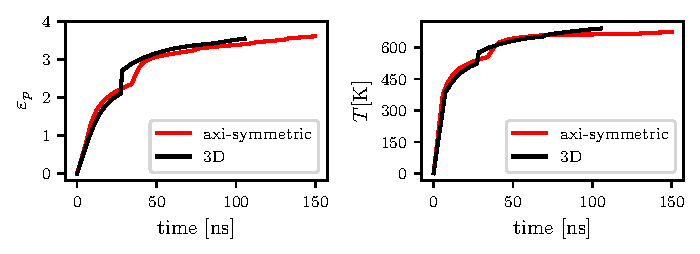
\includegraphics{cold-spray-plots}
  \caption{A PDF figure of which the font nearly matches the text font: 
  evolution of plastic strain $\varepsilon_p$ and temperature $T$ in time.}
  \label{fig:cold-spray-plot}
\end{figure}

\begin{figure}[!h]
  \centering
  %% Creator: Matplotlib, PGF backend
%%
%% To include the figure in your LaTeX document, write
%%   \input{<filename>.pgf}
%%
%% Make sure the required packages are loaded in your preamble
%%   \usepackage{pgf}
%%
%% Figures using additional raster images can only be included by \input if
%% they are in the same directory as the main LaTeX file. For loading figures
%% from other directories you can use the `import` package
%%   \usepackage{import}
%% and then include the figures with
%%   \import{<path to file>}{<filename>.pgf}
%%
%% Matplotlib used the following preamble
%%   \usepackage[utf8x]{inputenc}
%%   \usepackage[T1]{fontenc}
%%   \newcommand{\vect}[1]{#1}
%%
\begingroup%
\makeatletter%
\begin{pgfpicture}%
\pgfpathrectangle{\pgfpointorigin}{\pgfqpoint{6.375716in}{2.328394in}}%
\pgfusepath{use as bounding box, clip}%
\begin{pgfscope}%
\pgfsetbuttcap%
\pgfsetmiterjoin%
\definecolor{currentfill}{rgb}{1.000000,1.000000,1.000000}%
\pgfsetfillcolor{currentfill}%
\pgfsetlinewidth{0.000000pt}%
\definecolor{currentstroke}{rgb}{1.000000,1.000000,1.000000}%
\pgfsetstrokecolor{currentstroke}%
\pgfsetdash{}{0pt}%
\pgfpathmoveto{\pgfqpoint{0.000000in}{0.000000in}}%
\pgfpathlineto{\pgfqpoint{6.375716in}{0.000000in}}%
\pgfpathlineto{\pgfqpoint{6.375716in}{2.328394in}}%
\pgfpathlineto{\pgfqpoint{0.000000in}{2.328394in}}%
\pgfpathclose%
\pgfusepath{fill}%
\end{pgfscope}%
\begin{pgfscope}%
\pgfsetbuttcap%
\pgfsetmiterjoin%
\definecolor{currentfill}{rgb}{1.000000,1.000000,1.000000}%
\pgfsetfillcolor{currentfill}%
\pgfsetlinewidth{0.000000pt}%
\definecolor{currentstroke}{rgb}{0.000000,0.000000,0.000000}%
\pgfsetstrokecolor{currentstroke}%
\pgfsetstrokeopacity{0.000000}%
\pgfsetdash{}{0pt}%
\pgfpathmoveto{\pgfqpoint{0.434462in}{0.489757in}}%
\pgfpathlineto{\pgfqpoint{3.045729in}{0.489757in}}%
\pgfpathlineto{\pgfqpoint{3.045729in}{2.190131in}}%
\pgfpathlineto{\pgfqpoint{0.434462in}{2.190131in}}%
\pgfpathclose%
\pgfusepath{fill}%
\end{pgfscope}%
\begin{pgfscope}%
\pgfsetbuttcap%
\pgfsetroundjoin%
\definecolor{currentfill}{rgb}{0.000000,0.000000,0.000000}%
\pgfsetfillcolor{currentfill}%
\pgfsetlinewidth{0.803000pt}%
\definecolor{currentstroke}{rgb}{0.000000,0.000000,0.000000}%
\pgfsetstrokecolor{currentstroke}%
\pgfsetdash{}{0pt}%
\pgfsys@defobject{currentmarker}{\pgfqpoint{0.000000in}{-0.048611in}}{\pgfqpoint{0.000000in}{0.000000in}}{%
\pgfpathmoveto{\pgfqpoint{0.000000in}{0.000000in}}%
\pgfpathlineto{\pgfqpoint{0.000000in}{-0.048611in}}%
\pgfusepath{stroke,fill}%
}%
\begin{pgfscope}%
\pgfsys@transformshift{0.553156in}{0.489757in}%
\pgfsys@useobject{currentmarker}{}%
\end{pgfscope}%
\end{pgfscope}%
\begin{pgfscope}%
\definecolor{textcolor}{rgb}{0.000000,0.000000,0.000000}%
\pgfsetstrokecolor{textcolor}%
\pgfsetfillcolor{textcolor}%
\pgftext[x=0.553156in,y=0.392535in,,top]{\color{textcolor}\rmfamily\fontsize{8.000000}{9.600000}\selectfont \(\displaystyle 0\)}%
\end{pgfscope}%
\begin{pgfscope}%
\pgfsetbuttcap%
\pgfsetroundjoin%
\definecolor{currentfill}{rgb}{0.000000,0.000000,0.000000}%
\pgfsetfillcolor{currentfill}%
\pgfsetlinewidth{0.803000pt}%
\definecolor{currentstroke}{rgb}{0.000000,0.000000,0.000000}%
\pgfsetstrokecolor{currentstroke}%
\pgfsetdash{}{0pt}%
\pgfsys@defobject{currentmarker}{\pgfqpoint{0.000000in}{-0.048611in}}{\pgfqpoint{0.000000in}{0.000000in}}{%
\pgfpathmoveto{\pgfqpoint{0.000000in}{0.000000in}}%
\pgfpathlineto{\pgfqpoint{0.000000in}{-0.048611in}}%
\pgfusepath{stroke,fill}%
}%
\begin{pgfscope}%
\pgfsys@transformshift{0.948881in}{0.489757in}%
\pgfsys@useobject{currentmarker}{}%
\end{pgfscope}%
\end{pgfscope}%
\begin{pgfscope}%
\definecolor{textcolor}{rgb}{0.000000,0.000000,0.000000}%
\pgfsetstrokecolor{textcolor}%
\pgfsetfillcolor{textcolor}%
\pgftext[x=0.948881in,y=0.392535in,,top]{\color{textcolor}\rmfamily\fontsize{8.000000}{9.600000}\selectfont \(\displaystyle 25\)}%
\end{pgfscope}%
\begin{pgfscope}%
\pgfsetbuttcap%
\pgfsetroundjoin%
\definecolor{currentfill}{rgb}{0.000000,0.000000,0.000000}%
\pgfsetfillcolor{currentfill}%
\pgfsetlinewidth{0.803000pt}%
\definecolor{currentstroke}{rgb}{0.000000,0.000000,0.000000}%
\pgfsetstrokecolor{currentstroke}%
\pgfsetdash{}{0pt}%
\pgfsys@defobject{currentmarker}{\pgfqpoint{0.000000in}{-0.048611in}}{\pgfqpoint{0.000000in}{0.000000in}}{%
\pgfpathmoveto{\pgfqpoint{0.000000in}{0.000000in}}%
\pgfpathlineto{\pgfqpoint{0.000000in}{-0.048611in}}%
\pgfusepath{stroke,fill}%
}%
\begin{pgfscope}%
\pgfsys@transformshift{1.344607in}{0.489757in}%
\pgfsys@useobject{currentmarker}{}%
\end{pgfscope}%
\end{pgfscope}%
\begin{pgfscope}%
\definecolor{textcolor}{rgb}{0.000000,0.000000,0.000000}%
\pgfsetstrokecolor{textcolor}%
\pgfsetfillcolor{textcolor}%
\pgftext[x=1.344607in,y=0.392535in,,top]{\color{textcolor}\rmfamily\fontsize{8.000000}{9.600000}\selectfont \(\displaystyle 50\)}%
\end{pgfscope}%
\begin{pgfscope}%
\pgfsetbuttcap%
\pgfsetroundjoin%
\definecolor{currentfill}{rgb}{0.000000,0.000000,0.000000}%
\pgfsetfillcolor{currentfill}%
\pgfsetlinewidth{0.803000pt}%
\definecolor{currentstroke}{rgb}{0.000000,0.000000,0.000000}%
\pgfsetstrokecolor{currentstroke}%
\pgfsetdash{}{0pt}%
\pgfsys@defobject{currentmarker}{\pgfqpoint{0.000000in}{-0.048611in}}{\pgfqpoint{0.000000in}{0.000000in}}{%
\pgfpathmoveto{\pgfqpoint{0.000000in}{0.000000in}}%
\pgfpathlineto{\pgfqpoint{0.000000in}{-0.048611in}}%
\pgfusepath{stroke,fill}%
}%
\begin{pgfscope}%
\pgfsys@transformshift{1.740333in}{0.489757in}%
\pgfsys@useobject{currentmarker}{}%
\end{pgfscope}%
\end{pgfscope}%
\begin{pgfscope}%
\definecolor{textcolor}{rgb}{0.000000,0.000000,0.000000}%
\pgfsetstrokecolor{textcolor}%
\pgfsetfillcolor{textcolor}%
\pgftext[x=1.740333in,y=0.392535in,,top]{\color{textcolor}\rmfamily\fontsize{8.000000}{9.600000}\selectfont \(\displaystyle 75\)}%
\end{pgfscope}%
\begin{pgfscope}%
\pgfsetbuttcap%
\pgfsetroundjoin%
\definecolor{currentfill}{rgb}{0.000000,0.000000,0.000000}%
\pgfsetfillcolor{currentfill}%
\pgfsetlinewidth{0.803000pt}%
\definecolor{currentstroke}{rgb}{0.000000,0.000000,0.000000}%
\pgfsetstrokecolor{currentstroke}%
\pgfsetdash{}{0pt}%
\pgfsys@defobject{currentmarker}{\pgfqpoint{0.000000in}{-0.048611in}}{\pgfqpoint{0.000000in}{0.000000in}}{%
\pgfpathmoveto{\pgfqpoint{0.000000in}{0.000000in}}%
\pgfpathlineto{\pgfqpoint{0.000000in}{-0.048611in}}%
\pgfusepath{stroke,fill}%
}%
\begin{pgfscope}%
\pgfsys@transformshift{2.136059in}{0.489757in}%
\pgfsys@useobject{currentmarker}{}%
\end{pgfscope}%
\end{pgfscope}%
\begin{pgfscope}%
\definecolor{textcolor}{rgb}{0.000000,0.000000,0.000000}%
\pgfsetstrokecolor{textcolor}%
\pgfsetfillcolor{textcolor}%
\pgftext[x=2.136059in,y=0.392535in,,top]{\color{textcolor}\rmfamily\fontsize{8.000000}{9.600000}\selectfont \(\displaystyle 100\)}%
\end{pgfscope}%
\begin{pgfscope}%
\pgfsetbuttcap%
\pgfsetroundjoin%
\definecolor{currentfill}{rgb}{0.000000,0.000000,0.000000}%
\pgfsetfillcolor{currentfill}%
\pgfsetlinewidth{0.803000pt}%
\definecolor{currentstroke}{rgb}{0.000000,0.000000,0.000000}%
\pgfsetstrokecolor{currentstroke}%
\pgfsetdash{}{0pt}%
\pgfsys@defobject{currentmarker}{\pgfqpoint{0.000000in}{-0.048611in}}{\pgfqpoint{0.000000in}{0.000000in}}{%
\pgfpathmoveto{\pgfqpoint{0.000000in}{0.000000in}}%
\pgfpathlineto{\pgfqpoint{0.000000in}{-0.048611in}}%
\pgfusepath{stroke,fill}%
}%
\begin{pgfscope}%
\pgfsys@transformshift{2.531785in}{0.489757in}%
\pgfsys@useobject{currentmarker}{}%
\end{pgfscope}%
\end{pgfscope}%
\begin{pgfscope}%
\definecolor{textcolor}{rgb}{0.000000,0.000000,0.000000}%
\pgfsetstrokecolor{textcolor}%
\pgfsetfillcolor{textcolor}%
\pgftext[x=2.531785in,y=0.392535in,,top]{\color{textcolor}\rmfamily\fontsize{8.000000}{9.600000}\selectfont \(\displaystyle 125\)}%
\end{pgfscope}%
\begin{pgfscope}%
\pgfsetbuttcap%
\pgfsetroundjoin%
\definecolor{currentfill}{rgb}{0.000000,0.000000,0.000000}%
\pgfsetfillcolor{currentfill}%
\pgfsetlinewidth{0.803000pt}%
\definecolor{currentstroke}{rgb}{0.000000,0.000000,0.000000}%
\pgfsetstrokecolor{currentstroke}%
\pgfsetdash{}{0pt}%
\pgfsys@defobject{currentmarker}{\pgfqpoint{0.000000in}{-0.048611in}}{\pgfqpoint{0.000000in}{0.000000in}}{%
\pgfpathmoveto{\pgfqpoint{0.000000in}{0.000000in}}%
\pgfpathlineto{\pgfqpoint{0.000000in}{-0.048611in}}%
\pgfusepath{stroke,fill}%
}%
\begin{pgfscope}%
\pgfsys@transformshift{2.927510in}{0.489757in}%
\pgfsys@useobject{currentmarker}{}%
\end{pgfscope}%
\end{pgfscope}%
\begin{pgfscope}%
\definecolor{textcolor}{rgb}{0.000000,0.000000,0.000000}%
\pgfsetstrokecolor{textcolor}%
\pgfsetfillcolor{textcolor}%
\pgftext[x=2.927510in,y=0.392535in,,top]{\color{textcolor}\rmfamily\fontsize{8.000000}{9.600000}\selectfont \(\displaystyle 150\)}%
\end{pgfscope}%
\begin{pgfscope}%
\definecolor{textcolor}{rgb}{0.000000,0.000000,0.000000}%
\pgfsetstrokecolor{textcolor}%
\pgfsetfillcolor{textcolor}%
\pgftext[x=1.740096in,y=0.238855in,,top]{\color{textcolor}\rmfamily\fontsize{10.000000}{12.000000}\selectfont time [ns]}%
\end{pgfscope}%
\begin{pgfscope}%
\pgfsetbuttcap%
\pgfsetroundjoin%
\definecolor{currentfill}{rgb}{0.000000,0.000000,0.000000}%
\pgfsetfillcolor{currentfill}%
\pgfsetlinewidth{0.803000pt}%
\definecolor{currentstroke}{rgb}{0.000000,0.000000,0.000000}%
\pgfsetstrokecolor{currentstroke}%
\pgfsetdash{}{0pt}%
\pgfsys@defobject{currentmarker}{\pgfqpoint{-0.048611in}{0.000000in}}{\pgfqpoint{0.000000in}{0.000000in}}{%
\pgfpathmoveto{\pgfqpoint{0.000000in}{0.000000in}}%
\pgfpathlineto{\pgfqpoint{-0.048611in}{0.000000in}}%
\pgfusepath{stroke,fill}%
}%
\begin{pgfscope}%
\pgfsys@transformshift{0.434462in}{0.563078in}%
\pgfsys@useobject{currentmarker}{}%
\end{pgfscope}%
\end{pgfscope}%
\begin{pgfscope}%
\definecolor{textcolor}{rgb}{0.000000,0.000000,0.000000}%
\pgfsetstrokecolor{textcolor}%
\pgfsetfillcolor{textcolor}%
\pgftext[x=0.278211in,y=0.524816in,left,base]{\color{textcolor}\rmfamily\fontsize{8.000000}{9.600000}\selectfont \(\displaystyle 0\)}%
\end{pgfscope}%
\begin{pgfscope}%
\pgfsetbuttcap%
\pgfsetroundjoin%
\definecolor{currentfill}{rgb}{0.000000,0.000000,0.000000}%
\pgfsetfillcolor{currentfill}%
\pgfsetlinewidth{0.803000pt}%
\definecolor{currentstroke}{rgb}{0.000000,0.000000,0.000000}%
\pgfsetstrokecolor{currentstroke}%
\pgfsetdash{}{0pt}%
\pgfsys@defobject{currentmarker}{\pgfqpoint{-0.048611in}{0.000000in}}{\pgfqpoint{0.000000in}{0.000000in}}{%
\pgfpathmoveto{\pgfqpoint{0.000000in}{0.000000in}}%
\pgfpathlineto{\pgfqpoint{-0.048611in}{0.000000in}}%
\pgfusepath{stroke,fill}%
}%
\begin{pgfscope}%
\pgfsys@transformshift{0.434462in}{0.969841in}%
\pgfsys@useobject{currentmarker}{}%
\end{pgfscope}%
\end{pgfscope}%
\begin{pgfscope}%
\definecolor{textcolor}{rgb}{0.000000,0.000000,0.000000}%
\pgfsetstrokecolor{textcolor}%
\pgfsetfillcolor{textcolor}%
\pgftext[x=0.278211in,y=0.931579in,left,base]{\color{textcolor}\rmfamily\fontsize{8.000000}{9.600000}\selectfont \(\displaystyle 1\)}%
\end{pgfscope}%
\begin{pgfscope}%
\pgfsetbuttcap%
\pgfsetroundjoin%
\definecolor{currentfill}{rgb}{0.000000,0.000000,0.000000}%
\pgfsetfillcolor{currentfill}%
\pgfsetlinewidth{0.803000pt}%
\definecolor{currentstroke}{rgb}{0.000000,0.000000,0.000000}%
\pgfsetstrokecolor{currentstroke}%
\pgfsetdash{}{0pt}%
\pgfsys@defobject{currentmarker}{\pgfqpoint{-0.048611in}{0.000000in}}{\pgfqpoint{0.000000in}{0.000000in}}{%
\pgfpathmoveto{\pgfqpoint{0.000000in}{0.000000in}}%
\pgfpathlineto{\pgfqpoint{-0.048611in}{0.000000in}}%
\pgfusepath{stroke,fill}%
}%
\begin{pgfscope}%
\pgfsys@transformshift{0.434462in}{1.376605in}%
\pgfsys@useobject{currentmarker}{}%
\end{pgfscope}%
\end{pgfscope}%
\begin{pgfscope}%
\definecolor{textcolor}{rgb}{0.000000,0.000000,0.000000}%
\pgfsetstrokecolor{textcolor}%
\pgfsetfillcolor{textcolor}%
\pgftext[x=0.278211in,y=1.338342in,left,base]{\color{textcolor}\rmfamily\fontsize{8.000000}{9.600000}\selectfont \(\displaystyle 2\)}%
\end{pgfscope}%
\begin{pgfscope}%
\pgfsetbuttcap%
\pgfsetroundjoin%
\definecolor{currentfill}{rgb}{0.000000,0.000000,0.000000}%
\pgfsetfillcolor{currentfill}%
\pgfsetlinewidth{0.803000pt}%
\definecolor{currentstroke}{rgb}{0.000000,0.000000,0.000000}%
\pgfsetstrokecolor{currentstroke}%
\pgfsetdash{}{0pt}%
\pgfsys@defobject{currentmarker}{\pgfqpoint{-0.048611in}{0.000000in}}{\pgfqpoint{0.000000in}{0.000000in}}{%
\pgfpathmoveto{\pgfqpoint{0.000000in}{0.000000in}}%
\pgfpathlineto{\pgfqpoint{-0.048611in}{0.000000in}}%
\pgfusepath{stroke,fill}%
}%
\begin{pgfscope}%
\pgfsys@transformshift{0.434462in}{1.783368in}%
\pgfsys@useobject{currentmarker}{}%
\end{pgfscope}%
\end{pgfscope}%
\begin{pgfscope}%
\definecolor{textcolor}{rgb}{0.000000,0.000000,0.000000}%
\pgfsetstrokecolor{textcolor}%
\pgfsetfillcolor{textcolor}%
\pgftext[x=0.278211in,y=1.745106in,left,base]{\color{textcolor}\rmfamily\fontsize{8.000000}{9.600000}\selectfont \(\displaystyle 3\)}%
\end{pgfscope}%
\begin{pgfscope}%
\pgfsetbuttcap%
\pgfsetroundjoin%
\definecolor{currentfill}{rgb}{0.000000,0.000000,0.000000}%
\pgfsetfillcolor{currentfill}%
\pgfsetlinewidth{0.803000pt}%
\definecolor{currentstroke}{rgb}{0.000000,0.000000,0.000000}%
\pgfsetstrokecolor{currentstroke}%
\pgfsetdash{}{0pt}%
\pgfsys@defobject{currentmarker}{\pgfqpoint{-0.048611in}{0.000000in}}{\pgfqpoint{0.000000in}{0.000000in}}{%
\pgfpathmoveto{\pgfqpoint{0.000000in}{0.000000in}}%
\pgfpathlineto{\pgfqpoint{-0.048611in}{0.000000in}}%
\pgfusepath{stroke,fill}%
}%
\begin{pgfscope}%
\pgfsys@transformshift{0.434462in}{2.190131in}%
\pgfsys@useobject{currentmarker}{}%
\end{pgfscope}%
\end{pgfscope}%
\begin{pgfscope}%
\definecolor{textcolor}{rgb}{0.000000,0.000000,0.000000}%
\pgfsetstrokecolor{textcolor}%
\pgfsetfillcolor{textcolor}%
\pgftext[x=0.278211in,y=2.151869in,left,base]{\color{textcolor}\rmfamily\fontsize{8.000000}{9.600000}\selectfont \(\displaystyle 4\)}%
\end{pgfscope}%
\begin{pgfscope}%
\definecolor{textcolor}{rgb}{0.000000,0.000000,0.000000}%
\pgfsetstrokecolor{textcolor}%
\pgfsetfillcolor{textcolor}%
\pgftext[x=0.222655in,y=1.339944in,,bottom,rotate=90.000000]{\color{textcolor}\rmfamily\fontsize{10.000000}{12.000000}\selectfont \(\displaystyle \varepsilon_p\)}%
\end{pgfscope}%
\begin{pgfscope}%
\pgfpathrectangle{\pgfqpoint{0.434462in}{0.489757in}}{\pgfqpoint{2.611268in}{1.700374in}}%
\pgfusepath{clip}%
\pgfsetrectcap%
\pgfsetroundjoin%
\pgfsetlinewidth{1.505625pt}%
\definecolor{currentstroke}{rgb}{1.000000,0.000000,0.000000}%
\pgfsetstrokecolor{currentstroke}%
\pgfsetdash{}{0pt}%
\pgfpathmoveto{\pgfqpoint{0.553156in}{0.563078in}}%
\pgfpathlineto{\pgfqpoint{0.644136in}{0.898446in}}%
\pgfpathlineto{\pgfqpoint{0.677856in}{1.049453in}}%
\pgfpathlineto{\pgfqpoint{0.701275in}{1.128621in}}%
\pgfpathlineto{\pgfqpoint{0.720070in}{1.178198in}}%
\pgfpathlineto{\pgfqpoint{0.750463in}{1.247038in}}%
\pgfpathlineto{\pgfqpoint{0.763527in}{1.269512in}}%
\pgfpathlineto{\pgfqpoint{0.787471in}{1.301349in}}%
\pgfpathlineto{\pgfqpoint{0.819226in}{1.343112in}}%
\pgfpathlineto{\pgfqpoint{0.838567in}{1.361445in}}%
\pgfpathlineto{\pgfqpoint{0.899727in}{1.413807in}}%
\pgfpathlineto{\pgfqpoint{0.923829in}{1.429057in}}%
\pgfpathlineto{\pgfqpoint{0.946966in}{1.443696in}}%
\pgfpathlineto{\pgfqpoint{0.961875in}{1.454223in}}%
\pgfpathlineto{\pgfqpoint{0.983819in}{1.465991in}}%
\pgfpathlineto{\pgfqpoint{1.019222in}{1.483819in}}%
\pgfpathlineto{\pgfqpoint{1.032951in}{1.491572in}}%
\pgfpathlineto{\pgfqpoint{1.053315in}{1.500452in}}%
\pgfpathlineto{\pgfqpoint{1.086542in}{1.514200in}}%
\pgfpathlineto{\pgfqpoint{1.093049in}{1.517463in}}%
\pgfpathlineto{\pgfqpoint{1.099529in}{1.524715in}}%
\pgfpathlineto{\pgfqpoint{1.125278in}{1.594898in}}%
\pgfpathlineto{\pgfqpoint{1.144395in}{1.640806in}}%
\pgfpathlineto{\pgfqpoint{1.163208in}{1.678936in}}%
\pgfpathlineto{\pgfqpoint{1.181844in}{1.710216in}}%
\pgfpathlineto{\pgfqpoint{1.194230in}{1.728805in}}%
\pgfpathlineto{\pgfqpoint{1.206584in}{1.743741in}}%
\pgfpathlineto{\pgfqpoint{1.218857in}{1.753093in}}%
\pgfpathlineto{\pgfqpoint{1.254602in}{1.776233in}}%
\pgfpathlineto{\pgfqpoint{1.272082in}{1.786492in}}%
\pgfpathlineto{\pgfqpoint{1.289316in}{1.793944in}}%
\pgfpathlineto{\pgfqpoint{1.322880in}{1.804577in}}%
\pgfpathlineto{\pgfqpoint{1.361164in}{1.814729in}}%
\pgfpathlineto{\pgfqpoint{1.461503in}{1.836996in}}%
\pgfpathlineto{\pgfqpoint{1.523974in}{1.848283in}}%
\pgfpathlineto{\pgfqpoint{1.581436in}{1.856642in}}%
\pgfpathlineto{\pgfqpoint{1.655624in}{1.867027in}}%
\pgfpathlineto{\pgfqpoint{1.704159in}{1.877143in}}%
\pgfpathlineto{\pgfqpoint{1.720447in}{1.882065in}}%
\pgfpathlineto{\pgfqpoint{1.731353in}{1.887589in}}%
\pgfpathlineto{\pgfqpoint{1.736822in}{1.894923in}}%
\pgfpathlineto{\pgfqpoint{1.792102in}{1.902875in}}%
\pgfpathlineto{\pgfqpoint{1.888103in}{1.914395in}}%
\pgfpathlineto{\pgfqpoint{1.974797in}{1.922213in}}%
\pgfpathlineto{\pgfqpoint{2.105240in}{1.933289in}}%
\pgfpathlineto{\pgfqpoint{2.269941in}{1.950580in}}%
\pgfpathlineto{\pgfqpoint{2.307076in}{1.956071in}}%
\pgfpathlineto{\pgfqpoint{2.325738in}{1.960619in}}%
\pgfpathlineto{\pgfqpoint{2.338211in}{1.967221in}}%
\pgfpathlineto{\pgfqpoint{2.438726in}{1.974868in}}%
\pgfpathlineto{\pgfqpoint{2.598203in}{1.991277in}}%
\pgfpathlineto{\pgfqpoint{2.630368in}{1.996601in}}%
\pgfpathlineto{\pgfqpoint{2.643253in}{2.001076in}}%
\pgfpathlineto{\pgfqpoint{2.649711in}{2.006563in}}%
\pgfpathlineto{\pgfqpoint{2.830542in}{2.022651in}}%
\pgfpathlineto{\pgfqpoint{2.927035in}{2.029496in}}%
\pgfpathlineto{\pgfqpoint{2.927035in}{2.029496in}}%
\pgfusepath{stroke}%
\end{pgfscope}%
\begin{pgfscope}%
\pgfsetrectcap%
\pgfsetmiterjoin%
\pgfsetlinewidth{0.803000pt}%
\definecolor{currentstroke}{rgb}{0.000000,0.000000,0.000000}%
\pgfsetstrokecolor{currentstroke}%
\pgfsetdash{}{0pt}%
\pgfpathmoveto{\pgfqpoint{0.434462in}{0.489757in}}%
\pgfpathlineto{\pgfqpoint{0.434462in}{2.190131in}}%
\pgfusepath{stroke}%
\end{pgfscope}%
\begin{pgfscope}%
\pgfsetrectcap%
\pgfsetmiterjoin%
\pgfsetlinewidth{0.803000pt}%
\definecolor{currentstroke}{rgb}{0.000000,0.000000,0.000000}%
\pgfsetstrokecolor{currentstroke}%
\pgfsetdash{}{0pt}%
\pgfpathmoveto{\pgfqpoint{3.045729in}{0.489757in}}%
\pgfpathlineto{\pgfqpoint{3.045729in}{2.190131in}}%
\pgfusepath{stroke}%
\end{pgfscope}%
\begin{pgfscope}%
\pgfsetrectcap%
\pgfsetmiterjoin%
\pgfsetlinewidth{0.803000pt}%
\definecolor{currentstroke}{rgb}{0.000000,0.000000,0.000000}%
\pgfsetstrokecolor{currentstroke}%
\pgfsetdash{}{0pt}%
\pgfpathmoveto{\pgfqpoint{0.434462in}{0.489757in}}%
\pgfpathlineto{\pgfqpoint{3.045729in}{0.489757in}}%
\pgfusepath{stroke}%
\end{pgfscope}%
\begin{pgfscope}%
\pgfsetrectcap%
\pgfsetmiterjoin%
\pgfsetlinewidth{0.803000pt}%
\definecolor{currentstroke}{rgb}{0.000000,0.000000,0.000000}%
\pgfsetstrokecolor{currentstroke}%
\pgfsetdash{}{0pt}%
\pgfpathmoveto{\pgfqpoint{0.434462in}{2.190131in}}%
\pgfpathlineto{\pgfqpoint{3.045729in}{2.190131in}}%
\pgfusepath{stroke}%
\end{pgfscope}%
\begin{pgfscope}%
\pgfsetbuttcap%
\pgfsetmiterjoin%
\definecolor{currentfill}{rgb}{1.000000,1.000000,1.000000}%
\pgfsetfillcolor{currentfill}%
\pgfsetfillopacity{0.800000}%
\pgfsetlinewidth{1.003750pt}%
\definecolor{currentstroke}{rgb}{0.800000,0.800000,0.800000}%
\pgfsetstrokecolor{currentstroke}%
\pgfsetstrokeopacity{0.800000}%
\pgfsetdash{}{0pt}%
\pgfpathmoveto{\pgfqpoint{0.512239in}{1.946309in}}%
\pgfpathlineto{\pgfqpoint{1.596378in}{1.946309in}}%
\pgfpathquadraticcurveto{\pgfqpoint{1.618601in}{1.946309in}}{\pgfqpoint{1.618601in}{1.968532in}}%
\pgfpathlineto{\pgfqpoint{1.618601in}{2.112353in}}%
\pgfpathquadraticcurveto{\pgfqpoint{1.618601in}{2.134576in}}{\pgfqpoint{1.596378in}{2.134576in}}%
\pgfpathlineto{\pgfqpoint{0.512239in}{2.134576in}}%
\pgfpathquadraticcurveto{\pgfqpoint{0.490017in}{2.134576in}}{\pgfqpoint{0.490017in}{2.112353in}}%
\pgfpathlineto{\pgfqpoint{0.490017in}{1.968532in}}%
\pgfpathquadraticcurveto{\pgfqpoint{0.490017in}{1.946309in}}{\pgfqpoint{0.512239in}{1.946309in}}%
\pgfpathclose%
\pgfusepath{stroke,fill}%
\end{pgfscope}%
\begin{pgfscope}%
\pgfsetrectcap%
\pgfsetroundjoin%
\pgfsetlinewidth{1.505625pt}%
\definecolor{currentstroke}{rgb}{1.000000,0.000000,0.000000}%
\pgfsetstrokecolor{currentstroke}%
\pgfsetdash{}{0pt}%
\pgfpathmoveto{\pgfqpoint{0.534462in}{2.051242in}}%
\pgfpathlineto{\pgfqpoint{0.756684in}{2.051242in}}%
\pgfusepath{stroke}%
\end{pgfscope}%
\begin{pgfscope}%
\definecolor{textcolor}{rgb}{0.000000,0.000000,0.000000}%
\pgfsetstrokecolor{textcolor}%
\pgfsetfillcolor{textcolor}%
\pgftext[x=0.845573in,y=2.012353in,left,base]{\color{textcolor}\rmfamily\fontsize{8.000000}{9.600000}\selectfont axi-symmetric}%
\end{pgfscope}%
\begin{pgfscope}%
\pgfsetbuttcap%
\pgfsetmiterjoin%
\definecolor{currentfill}{rgb}{1.000000,1.000000,1.000000}%
\pgfsetfillcolor{currentfill}%
\pgfsetlinewidth{0.000000pt}%
\definecolor{currentstroke}{rgb}{0.000000,0.000000,0.000000}%
\pgfsetstrokecolor{currentstroke}%
\pgfsetstrokeopacity{0.000000}%
\pgfsetdash{}{0pt}%
\pgfpathmoveto{\pgfqpoint{3.664448in}{0.489757in}}%
\pgfpathlineto{\pgfqpoint{6.275716in}{0.489757in}}%
\pgfpathlineto{\pgfqpoint{6.275716in}{2.190131in}}%
\pgfpathlineto{\pgfqpoint{3.664448in}{2.190131in}}%
\pgfpathclose%
\pgfusepath{fill}%
\end{pgfscope}%
\begin{pgfscope}%
\pgfsetbuttcap%
\pgfsetroundjoin%
\definecolor{currentfill}{rgb}{0.000000,0.000000,0.000000}%
\pgfsetfillcolor{currentfill}%
\pgfsetlinewidth{0.803000pt}%
\definecolor{currentstroke}{rgb}{0.000000,0.000000,0.000000}%
\pgfsetstrokecolor{currentstroke}%
\pgfsetdash{}{0pt}%
\pgfsys@defobject{currentmarker}{\pgfqpoint{0.000000in}{-0.048611in}}{\pgfqpoint{0.000000in}{0.000000in}}{%
\pgfpathmoveto{\pgfqpoint{0.000000in}{0.000000in}}%
\pgfpathlineto{\pgfqpoint{0.000000in}{-0.048611in}}%
\pgfusepath{stroke,fill}%
}%
\begin{pgfscope}%
\pgfsys@transformshift{3.783142in}{0.489757in}%
\pgfsys@useobject{currentmarker}{}%
\end{pgfscope}%
\end{pgfscope}%
\begin{pgfscope}%
\definecolor{textcolor}{rgb}{0.000000,0.000000,0.000000}%
\pgfsetstrokecolor{textcolor}%
\pgfsetfillcolor{textcolor}%
\pgftext[x=3.783142in,y=0.392535in,,top]{\color{textcolor}\rmfamily\fontsize{8.000000}{9.600000}\selectfont \(\displaystyle 0\)}%
\end{pgfscope}%
\begin{pgfscope}%
\pgfsetbuttcap%
\pgfsetroundjoin%
\definecolor{currentfill}{rgb}{0.000000,0.000000,0.000000}%
\pgfsetfillcolor{currentfill}%
\pgfsetlinewidth{0.803000pt}%
\definecolor{currentstroke}{rgb}{0.000000,0.000000,0.000000}%
\pgfsetstrokecolor{currentstroke}%
\pgfsetdash{}{0pt}%
\pgfsys@defobject{currentmarker}{\pgfqpoint{0.000000in}{-0.048611in}}{\pgfqpoint{0.000000in}{0.000000in}}{%
\pgfpathmoveto{\pgfqpoint{0.000000in}{0.000000in}}%
\pgfpathlineto{\pgfqpoint{0.000000in}{-0.048611in}}%
\pgfusepath{stroke,fill}%
}%
\begin{pgfscope}%
\pgfsys@transformshift{4.178868in}{0.489757in}%
\pgfsys@useobject{currentmarker}{}%
\end{pgfscope}%
\end{pgfscope}%
\begin{pgfscope}%
\definecolor{textcolor}{rgb}{0.000000,0.000000,0.000000}%
\pgfsetstrokecolor{textcolor}%
\pgfsetfillcolor{textcolor}%
\pgftext[x=4.178868in,y=0.392535in,,top]{\color{textcolor}\rmfamily\fontsize{8.000000}{9.600000}\selectfont \(\displaystyle 25\)}%
\end{pgfscope}%
\begin{pgfscope}%
\pgfsetbuttcap%
\pgfsetroundjoin%
\definecolor{currentfill}{rgb}{0.000000,0.000000,0.000000}%
\pgfsetfillcolor{currentfill}%
\pgfsetlinewidth{0.803000pt}%
\definecolor{currentstroke}{rgb}{0.000000,0.000000,0.000000}%
\pgfsetstrokecolor{currentstroke}%
\pgfsetdash{}{0pt}%
\pgfsys@defobject{currentmarker}{\pgfqpoint{0.000000in}{-0.048611in}}{\pgfqpoint{0.000000in}{0.000000in}}{%
\pgfpathmoveto{\pgfqpoint{0.000000in}{0.000000in}}%
\pgfpathlineto{\pgfqpoint{0.000000in}{-0.048611in}}%
\pgfusepath{stroke,fill}%
}%
\begin{pgfscope}%
\pgfsys@transformshift{4.574594in}{0.489757in}%
\pgfsys@useobject{currentmarker}{}%
\end{pgfscope}%
\end{pgfscope}%
\begin{pgfscope}%
\definecolor{textcolor}{rgb}{0.000000,0.000000,0.000000}%
\pgfsetstrokecolor{textcolor}%
\pgfsetfillcolor{textcolor}%
\pgftext[x=4.574594in,y=0.392535in,,top]{\color{textcolor}\rmfamily\fontsize{8.000000}{9.600000}\selectfont \(\displaystyle 50\)}%
\end{pgfscope}%
\begin{pgfscope}%
\pgfsetbuttcap%
\pgfsetroundjoin%
\definecolor{currentfill}{rgb}{0.000000,0.000000,0.000000}%
\pgfsetfillcolor{currentfill}%
\pgfsetlinewidth{0.803000pt}%
\definecolor{currentstroke}{rgb}{0.000000,0.000000,0.000000}%
\pgfsetstrokecolor{currentstroke}%
\pgfsetdash{}{0pt}%
\pgfsys@defobject{currentmarker}{\pgfqpoint{0.000000in}{-0.048611in}}{\pgfqpoint{0.000000in}{0.000000in}}{%
\pgfpathmoveto{\pgfqpoint{0.000000in}{0.000000in}}%
\pgfpathlineto{\pgfqpoint{0.000000in}{-0.048611in}}%
\pgfusepath{stroke,fill}%
}%
\begin{pgfscope}%
\pgfsys@transformshift{4.970320in}{0.489757in}%
\pgfsys@useobject{currentmarker}{}%
\end{pgfscope}%
\end{pgfscope}%
\begin{pgfscope}%
\definecolor{textcolor}{rgb}{0.000000,0.000000,0.000000}%
\pgfsetstrokecolor{textcolor}%
\pgfsetfillcolor{textcolor}%
\pgftext[x=4.970320in,y=0.392535in,,top]{\color{textcolor}\rmfamily\fontsize{8.000000}{9.600000}\selectfont \(\displaystyle 75\)}%
\end{pgfscope}%
\begin{pgfscope}%
\pgfsetbuttcap%
\pgfsetroundjoin%
\definecolor{currentfill}{rgb}{0.000000,0.000000,0.000000}%
\pgfsetfillcolor{currentfill}%
\pgfsetlinewidth{0.803000pt}%
\definecolor{currentstroke}{rgb}{0.000000,0.000000,0.000000}%
\pgfsetstrokecolor{currentstroke}%
\pgfsetdash{}{0pt}%
\pgfsys@defobject{currentmarker}{\pgfqpoint{0.000000in}{-0.048611in}}{\pgfqpoint{0.000000in}{0.000000in}}{%
\pgfpathmoveto{\pgfqpoint{0.000000in}{0.000000in}}%
\pgfpathlineto{\pgfqpoint{0.000000in}{-0.048611in}}%
\pgfusepath{stroke,fill}%
}%
\begin{pgfscope}%
\pgfsys@transformshift{5.366045in}{0.489757in}%
\pgfsys@useobject{currentmarker}{}%
\end{pgfscope}%
\end{pgfscope}%
\begin{pgfscope}%
\definecolor{textcolor}{rgb}{0.000000,0.000000,0.000000}%
\pgfsetstrokecolor{textcolor}%
\pgfsetfillcolor{textcolor}%
\pgftext[x=5.366045in,y=0.392535in,,top]{\color{textcolor}\rmfamily\fontsize{8.000000}{9.600000}\selectfont \(\displaystyle 100\)}%
\end{pgfscope}%
\begin{pgfscope}%
\pgfsetbuttcap%
\pgfsetroundjoin%
\definecolor{currentfill}{rgb}{0.000000,0.000000,0.000000}%
\pgfsetfillcolor{currentfill}%
\pgfsetlinewidth{0.803000pt}%
\definecolor{currentstroke}{rgb}{0.000000,0.000000,0.000000}%
\pgfsetstrokecolor{currentstroke}%
\pgfsetdash{}{0pt}%
\pgfsys@defobject{currentmarker}{\pgfqpoint{0.000000in}{-0.048611in}}{\pgfqpoint{0.000000in}{0.000000in}}{%
\pgfpathmoveto{\pgfqpoint{0.000000in}{0.000000in}}%
\pgfpathlineto{\pgfqpoint{0.000000in}{-0.048611in}}%
\pgfusepath{stroke,fill}%
}%
\begin{pgfscope}%
\pgfsys@transformshift{5.761771in}{0.489757in}%
\pgfsys@useobject{currentmarker}{}%
\end{pgfscope}%
\end{pgfscope}%
\begin{pgfscope}%
\definecolor{textcolor}{rgb}{0.000000,0.000000,0.000000}%
\pgfsetstrokecolor{textcolor}%
\pgfsetfillcolor{textcolor}%
\pgftext[x=5.761771in,y=0.392535in,,top]{\color{textcolor}\rmfamily\fontsize{8.000000}{9.600000}\selectfont \(\displaystyle 125\)}%
\end{pgfscope}%
\begin{pgfscope}%
\pgfsetbuttcap%
\pgfsetroundjoin%
\definecolor{currentfill}{rgb}{0.000000,0.000000,0.000000}%
\pgfsetfillcolor{currentfill}%
\pgfsetlinewidth{0.803000pt}%
\definecolor{currentstroke}{rgb}{0.000000,0.000000,0.000000}%
\pgfsetstrokecolor{currentstroke}%
\pgfsetdash{}{0pt}%
\pgfsys@defobject{currentmarker}{\pgfqpoint{0.000000in}{-0.048611in}}{\pgfqpoint{0.000000in}{0.000000in}}{%
\pgfpathmoveto{\pgfqpoint{0.000000in}{0.000000in}}%
\pgfpathlineto{\pgfqpoint{0.000000in}{-0.048611in}}%
\pgfusepath{stroke,fill}%
}%
\begin{pgfscope}%
\pgfsys@transformshift{6.157497in}{0.489757in}%
\pgfsys@useobject{currentmarker}{}%
\end{pgfscope}%
\end{pgfscope}%
\begin{pgfscope}%
\definecolor{textcolor}{rgb}{0.000000,0.000000,0.000000}%
\pgfsetstrokecolor{textcolor}%
\pgfsetfillcolor{textcolor}%
\pgftext[x=6.157497in,y=0.392535in,,top]{\color{textcolor}\rmfamily\fontsize{8.000000}{9.600000}\selectfont \(\displaystyle 150\)}%
\end{pgfscope}%
\begin{pgfscope}%
\definecolor{textcolor}{rgb}{0.000000,0.000000,0.000000}%
\pgfsetstrokecolor{textcolor}%
\pgfsetfillcolor{textcolor}%
\pgftext[x=4.970082in,y=0.238855in,,top]{\color{textcolor}\rmfamily\fontsize{10.000000}{12.000000}\selectfont time [ns]}%
\end{pgfscope}%
\begin{pgfscope}%
\pgfsetbuttcap%
\pgfsetroundjoin%
\definecolor{currentfill}{rgb}{0.000000,0.000000,0.000000}%
\pgfsetfillcolor{currentfill}%
\pgfsetlinewidth{0.803000pt}%
\definecolor{currentstroke}{rgb}{0.000000,0.000000,0.000000}%
\pgfsetstrokecolor{currentstroke}%
\pgfsetdash{}{0pt}%
\pgfsys@defobject{currentmarker}{\pgfqpoint{-0.048611in}{0.000000in}}{\pgfqpoint{0.000000in}{0.000000in}}{%
\pgfpathmoveto{\pgfqpoint{0.000000in}{0.000000in}}%
\pgfpathlineto{\pgfqpoint{-0.048611in}{0.000000in}}%
\pgfusepath{stroke,fill}%
}%
\begin{pgfscope}%
\pgfsys@transformshift{3.664448in}{0.567047in}%
\pgfsys@useobject{currentmarker}{}%
\end{pgfscope}%
\end{pgfscope}%
\begin{pgfscope}%
\definecolor{textcolor}{rgb}{0.000000,0.000000,0.000000}%
\pgfsetstrokecolor{textcolor}%
\pgfsetfillcolor{textcolor}%
\pgftext[x=3.508197in,y=0.528785in,left,base]{\color{textcolor}\rmfamily\fontsize{8.000000}{9.600000}\selectfont \(\displaystyle 0\)}%
\end{pgfscope}%
\begin{pgfscope}%
\pgfsetbuttcap%
\pgfsetroundjoin%
\definecolor{currentfill}{rgb}{0.000000,0.000000,0.000000}%
\pgfsetfillcolor{currentfill}%
\pgfsetlinewidth{0.803000pt}%
\definecolor{currentstroke}{rgb}{0.000000,0.000000,0.000000}%
\pgfsetstrokecolor{currentstroke}%
\pgfsetdash{}{0pt}%
\pgfsys@defobject{currentmarker}{\pgfqpoint{-0.048611in}{0.000000in}}{\pgfqpoint{0.000000in}{0.000000in}}{%
\pgfpathmoveto{\pgfqpoint{0.000000in}{0.000000in}}%
\pgfpathlineto{\pgfqpoint{-0.048611in}{0.000000in}}%
\pgfusepath{stroke,fill}%
}%
\begin{pgfscope}%
\pgfsys@transformshift{3.664448in}{0.910917in}%
\pgfsys@useobject{currentmarker}{}%
\end{pgfscope}%
\end{pgfscope}%
\begin{pgfscope}%
\definecolor{textcolor}{rgb}{0.000000,0.000000,0.000000}%
\pgfsetstrokecolor{textcolor}%
\pgfsetfillcolor{textcolor}%
\pgftext[x=3.390140in,y=0.872655in,left,base]{\color{textcolor}\rmfamily\fontsize{8.000000}{9.600000}\selectfont \(\displaystyle 150\)}%
\end{pgfscope}%
\begin{pgfscope}%
\pgfsetbuttcap%
\pgfsetroundjoin%
\definecolor{currentfill}{rgb}{0.000000,0.000000,0.000000}%
\pgfsetfillcolor{currentfill}%
\pgfsetlinewidth{0.803000pt}%
\definecolor{currentstroke}{rgb}{0.000000,0.000000,0.000000}%
\pgfsetstrokecolor{currentstroke}%
\pgfsetdash{}{0pt}%
\pgfsys@defobject{currentmarker}{\pgfqpoint{-0.048611in}{0.000000in}}{\pgfqpoint{0.000000in}{0.000000in}}{%
\pgfpathmoveto{\pgfqpoint{0.000000in}{0.000000in}}%
\pgfpathlineto{\pgfqpoint{-0.048611in}{0.000000in}}%
\pgfusepath{stroke,fill}%
}%
\begin{pgfscope}%
\pgfsys@transformshift{3.664448in}{1.254788in}%
\pgfsys@useobject{currentmarker}{}%
\end{pgfscope}%
\end{pgfscope}%
\begin{pgfscope}%
\definecolor{textcolor}{rgb}{0.000000,0.000000,0.000000}%
\pgfsetstrokecolor{textcolor}%
\pgfsetfillcolor{textcolor}%
\pgftext[x=3.390140in,y=1.216526in,left,base]{\color{textcolor}\rmfamily\fontsize{8.000000}{9.600000}\selectfont \(\displaystyle 300\)}%
\end{pgfscope}%
\begin{pgfscope}%
\pgfsetbuttcap%
\pgfsetroundjoin%
\definecolor{currentfill}{rgb}{0.000000,0.000000,0.000000}%
\pgfsetfillcolor{currentfill}%
\pgfsetlinewidth{0.803000pt}%
\definecolor{currentstroke}{rgb}{0.000000,0.000000,0.000000}%
\pgfsetstrokecolor{currentstroke}%
\pgfsetdash{}{0pt}%
\pgfsys@defobject{currentmarker}{\pgfqpoint{-0.048611in}{0.000000in}}{\pgfqpoint{0.000000in}{0.000000in}}{%
\pgfpathmoveto{\pgfqpoint{0.000000in}{0.000000in}}%
\pgfpathlineto{\pgfqpoint{-0.048611in}{0.000000in}}%
\pgfusepath{stroke,fill}%
}%
\begin{pgfscope}%
\pgfsys@transformshift{3.664448in}{1.598659in}%
\pgfsys@useobject{currentmarker}{}%
\end{pgfscope}%
\end{pgfscope}%
\begin{pgfscope}%
\definecolor{textcolor}{rgb}{0.000000,0.000000,0.000000}%
\pgfsetstrokecolor{textcolor}%
\pgfsetfillcolor{textcolor}%
\pgftext[x=3.390140in,y=1.560396in,left,base]{\color{textcolor}\rmfamily\fontsize{8.000000}{9.600000}\selectfont \(\displaystyle 450\)}%
\end{pgfscope}%
\begin{pgfscope}%
\pgfsetbuttcap%
\pgfsetroundjoin%
\definecolor{currentfill}{rgb}{0.000000,0.000000,0.000000}%
\pgfsetfillcolor{currentfill}%
\pgfsetlinewidth{0.803000pt}%
\definecolor{currentstroke}{rgb}{0.000000,0.000000,0.000000}%
\pgfsetstrokecolor{currentstroke}%
\pgfsetdash{}{0pt}%
\pgfsys@defobject{currentmarker}{\pgfqpoint{-0.048611in}{0.000000in}}{\pgfqpoint{0.000000in}{0.000000in}}{%
\pgfpathmoveto{\pgfqpoint{0.000000in}{0.000000in}}%
\pgfpathlineto{\pgfqpoint{-0.048611in}{0.000000in}}%
\pgfusepath{stroke,fill}%
}%
\begin{pgfscope}%
\pgfsys@transformshift{3.664448in}{1.942529in}%
\pgfsys@useobject{currentmarker}{}%
\end{pgfscope}%
\end{pgfscope}%
\begin{pgfscope}%
\definecolor{textcolor}{rgb}{0.000000,0.000000,0.000000}%
\pgfsetstrokecolor{textcolor}%
\pgfsetfillcolor{textcolor}%
\pgftext[x=3.390140in,y=1.904267in,left,base]{\color{textcolor}\rmfamily\fontsize{8.000000}{9.600000}\selectfont \(\displaystyle 600\)}%
\end{pgfscope}%
\begin{pgfscope}%
\definecolor{textcolor}{rgb}{0.000000,0.000000,0.000000}%
\pgfsetstrokecolor{textcolor}%
\pgfsetfillcolor{textcolor}%
\pgftext[x=3.334584in,y=1.339944in,,bottom,rotate=90.000000]{\color{textcolor}\rmfamily\fontsize{10.000000}{12.000000}\selectfont \(\displaystyle T\)[K]}%
\end{pgfscope}%
\begin{pgfscope}%
\pgfpathrectangle{\pgfqpoint{3.664448in}{0.489757in}}{\pgfqpoint{2.611268in}{1.700374in}}%
\pgfusepath{clip}%
\pgfsetrectcap%
\pgfsetroundjoin%
\pgfsetlinewidth{1.505625pt}%
\definecolor{currentstroke}{rgb}{1.000000,0.000000,0.000000}%
\pgfsetstrokecolor{currentstroke}%
\pgfsetdash{}{0pt}%
\pgfpathmoveto{\pgfqpoint{3.783142in}{0.567047in}}%
\pgfpathlineto{\pgfqpoint{3.874122in}{1.421471in}}%
\pgfpathlineto{\pgfqpoint{3.907842in}{1.519137in}}%
\pgfpathlineto{\pgfqpoint{3.931261in}{1.572217in}}%
\pgfpathlineto{\pgfqpoint{3.950056in}{1.605885in}}%
\pgfpathlineto{\pgfqpoint{3.980449in}{1.653013in}}%
\pgfpathlineto{\pgfqpoint{3.993513in}{1.668467in}}%
\pgfpathlineto{\pgfqpoint{4.017458in}{1.690401in}}%
\pgfpathlineto{\pgfqpoint{4.049212in}{1.719227in}}%
\pgfpathlineto{\pgfqpoint{4.077899in}{1.737986in}}%
\pgfpathlineto{\pgfqpoint{4.113158in}{1.758806in}}%
\pgfpathlineto{\pgfqpoint{4.129714in}{1.768535in}}%
\pgfpathlineto{\pgfqpoint{4.153815in}{1.779062in}}%
\pgfpathlineto{\pgfqpoint{4.176953in}{1.789170in}}%
\pgfpathlineto{\pgfqpoint{4.199224in}{1.799431in}}%
\pgfpathlineto{\pgfqpoint{4.269752in}{1.824387in}}%
\pgfpathlineto{\pgfqpoint{4.323036in}{1.839987in}}%
\pgfpathlineto{\pgfqpoint{4.329516in}{1.846908in}}%
\pgfpathlineto{\pgfqpoint{4.355265in}{1.895038in}}%
\pgfpathlineto{\pgfqpoint{4.374382in}{1.926363in}}%
\pgfpathlineto{\pgfqpoint{4.393195in}{1.952263in}}%
\pgfpathlineto{\pgfqpoint{4.411830in}{1.973420in}}%
\pgfpathlineto{\pgfqpoint{4.430399in}{1.991373in}}%
\pgfpathlineto{\pgfqpoint{4.442727in}{1.999495in}}%
\pgfpathlineto{\pgfqpoint{4.490439in}{2.020214in}}%
\pgfpathlineto{\pgfqpoint{4.513592in}{2.028183in}}%
\pgfpathlineto{\pgfqpoint{4.547333in}{2.035601in}}%
\pgfpathlineto{\pgfqpoint{4.596541in}{2.044269in}}%
\pgfpathlineto{\pgfqpoint{4.733099in}{2.063313in}}%
\pgfpathlineto{\pgfqpoint{4.811423in}{2.071164in}}%
\pgfpathlineto{\pgfqpoint{4.977781in}{2.084149in}}%
\pgfpathlineto{\pgfqpoint{5.675028in}{2.084841in}}%
\pgfpathlineto{\pgfqpoint{5.757751in}{2.090767in}}%
\pgfpathlineto{\pgfqpoint{6.079887in}{2.109339in}}%
\pgfpathlineto{\pgfqpoint{6.157022in}{2.112841in}}%
\pgfpathlineto{\pgfqpoint{6.157022in}{2.112841in}}%
\pgfusepath{stroke}%
\end{pgfscope}%
\begin{pgfscope}%
\pgfsetrectcap%
\pgfsetmiterjoin%
\pgfsetlinewidth{0.803000pt}%
\definecolor{currentstroke}{rgb}{0.000000,0.000000,0.000000}%
\pgfsetstrokecolor{currentstroke}%
\pgfsetdash{}{0pt}%
\pgfpathmoveto{\pgfqpoint{3.664448in}{0.489757in}}%
\pgfpathlineto{\pgfqpoint{3.664448in}{2.190131in}}%
\pgfusepath{stroke}%
\end{pgfscope}%
\begin{pgfscope}%
\pgfsetrectcap%
\pgfsetmiterjoin%
\pgfsetlinewidth{0.803000pt}%
\definecolor{currentstroke}{rgb}{0.000000,0.000000,0.000000}%
\pgfsetstrokecolor{currentstroke}%
\pgfsetdash{}{0pt}%
\pgfpathmoveto{\pgfqpoint{6.275716in}{0.489757in}}%
\pgfpathlineto{\pgfqpoint{6.275716in}{2.190131in}}%
\pgfusepath{stroke}%
\end{pgfscope}%
\begin{pgfscope}%
\pgfsetrectcap%
\pgfsetmiterjoin%
\pgfsetlinewidth{0.803000pt}%
\definecolor{currentstroke}{rgb}{0.000000,0.000000,0.000000}%
\pgfsetstrokecolor{currentstroke}%
\pgfsetdash{}{0pt}%
\pgfpathmoveto{\pgfqpoint{3.664448in}{0.489757in}}%
\pgfpathlineto{\pgfqpoint{6.275716in}{0.489757in}}%
\pgfusepath{stroke}%
\end{pgfscope}%
\begin{pgfscope}%
\pgfsetrectcap%
\pgfsetmiterjoin%
\pgfsetlinewidth{0.803000pt}%
\definecolor{currentstroke}{rgb}{0.000000,0.000000,0.000000}%
\pgfsetstrokecolor{currentstroke}%
\pgfsetdash{}{0pt}%
\pgfpathmoveto{\pgfqpoint{3.664448in}{2.190131in}}%
\pgfpathlineto{\pgfqpoint{6.275716in}{2.190131in}}%
\pgfusepath{stroke}%
\end{pgfscope}%
\begin{pgfscope}%
\pgfsetbuttcap%
\pgfsetmiterjoin%
\definecolor{currentfill}{rgb}{1.000000,1.000000,1.000000}%
\pgfsetfillcolor{currentfill}%
\pgfsetfillopacity{0.800000}%
\pgfsetlinewidth{1.003750pt}%
\definecolor{currentstroke}{rgb}{0.800000,0.800000,0.800000}%
\pgfsetstrokecolor{currentstroke}%
\pgfsetstrokeopacity{0.800000}%
\pgfsetdash{}{0pt}%
\pgfpathmoveto{\pgfqpoint{5.113799in}{0.545313in}}%
\pgfpathlineto{\pgfqpoint{6.197938in}{0.545313in}}%
\pgfpathquadraticcurveto{\pgfqpoint{6.220161in}{0.545313in}}{\pgfqpoint{6.220161in}{0.567535in}}%
\pgfpathlineto{\pgfqpoint{6.220161in}{0.711357in}}%
\pgfpathquadraticcurveto{\pgfqpoint{6.220161in}{0.733579in}}{\pgfqpoint{6.197938in}{0.733579in}}%
\pgfpathlineto{\pgfqpoint{5.113799in}{0.733579in}}%
\pgfpathquadraticcurveto{\pgfqpoint{5.091577in}{0.733579in}}{\pgfqpoint{5.091577in}{0.711357in}}%
\pgfpathlineto{\pgfqpoint{5.091577in}{0.567535in}}%
\pgfpathquadraticcurveto{\pgfqpoint{5.091577in}{0.545313in}}{\pgfqpoint{5.113799in}{0.545313in}}%
\pgfpathclose%
\pgfusepath{stroke,fill}%
\end{pgfscope}%
\begin{pgfscope}%
\pgfsetrectcap%
\pgfsetroundjoin%
\pgfsetlinewidth{1.505625pt}%
\definecolor{currentstroke}{rgb}{1.000000,0.000000,0.000000}%
\pgfsetstrokecolor{currentstroke}%
\pgfsetdash{}{0pt}%
\pgfpathmoveto{\pgfqpoint{5.136021in}{0.650246in}}%
\pgfpathlineto{\pgfqpoint{5.358244in}{0.650246in}}%
\pgfusepath{stroke}%
\end{pgfscope}%
\begin{pgfscope}%
\definecolor{textcolor}{rgb}{0.000000,0.000000,0.000000}%
\pgfsetstrokecolor{textcolor}%
\pgfsetfillcolor{textcolor}%
\pgftext[x=5.447132in,y=0.611357in,left,base]{\color{textcolor}\rmfamily\fontsize{8.000000}{9.600000}\selectfont axi-symmetric}%
\end{pgfscope}%
\end{pgfpicture}%
\makeatother%
\endgroup%

  \caption{A PGF figure of which the font matches the text font: 
  evolution of plastic strain $\varepsilon_p$ and temperature  $T$ in time.}
  \label{fig:cold-spray-plot-pgf}
\end{figure}


%---------------------------

If you want to stack multiple pictures together with sub-captions using \LaTeX\ the package \texttt{subfig} can do the job. \cref{fig:figures1} is a collection of 4 figures, with caption for each one. The \LaTeX\ code is given in \cref{snippet_sub_figures}.


\begin{figure}[!h]
  \centering
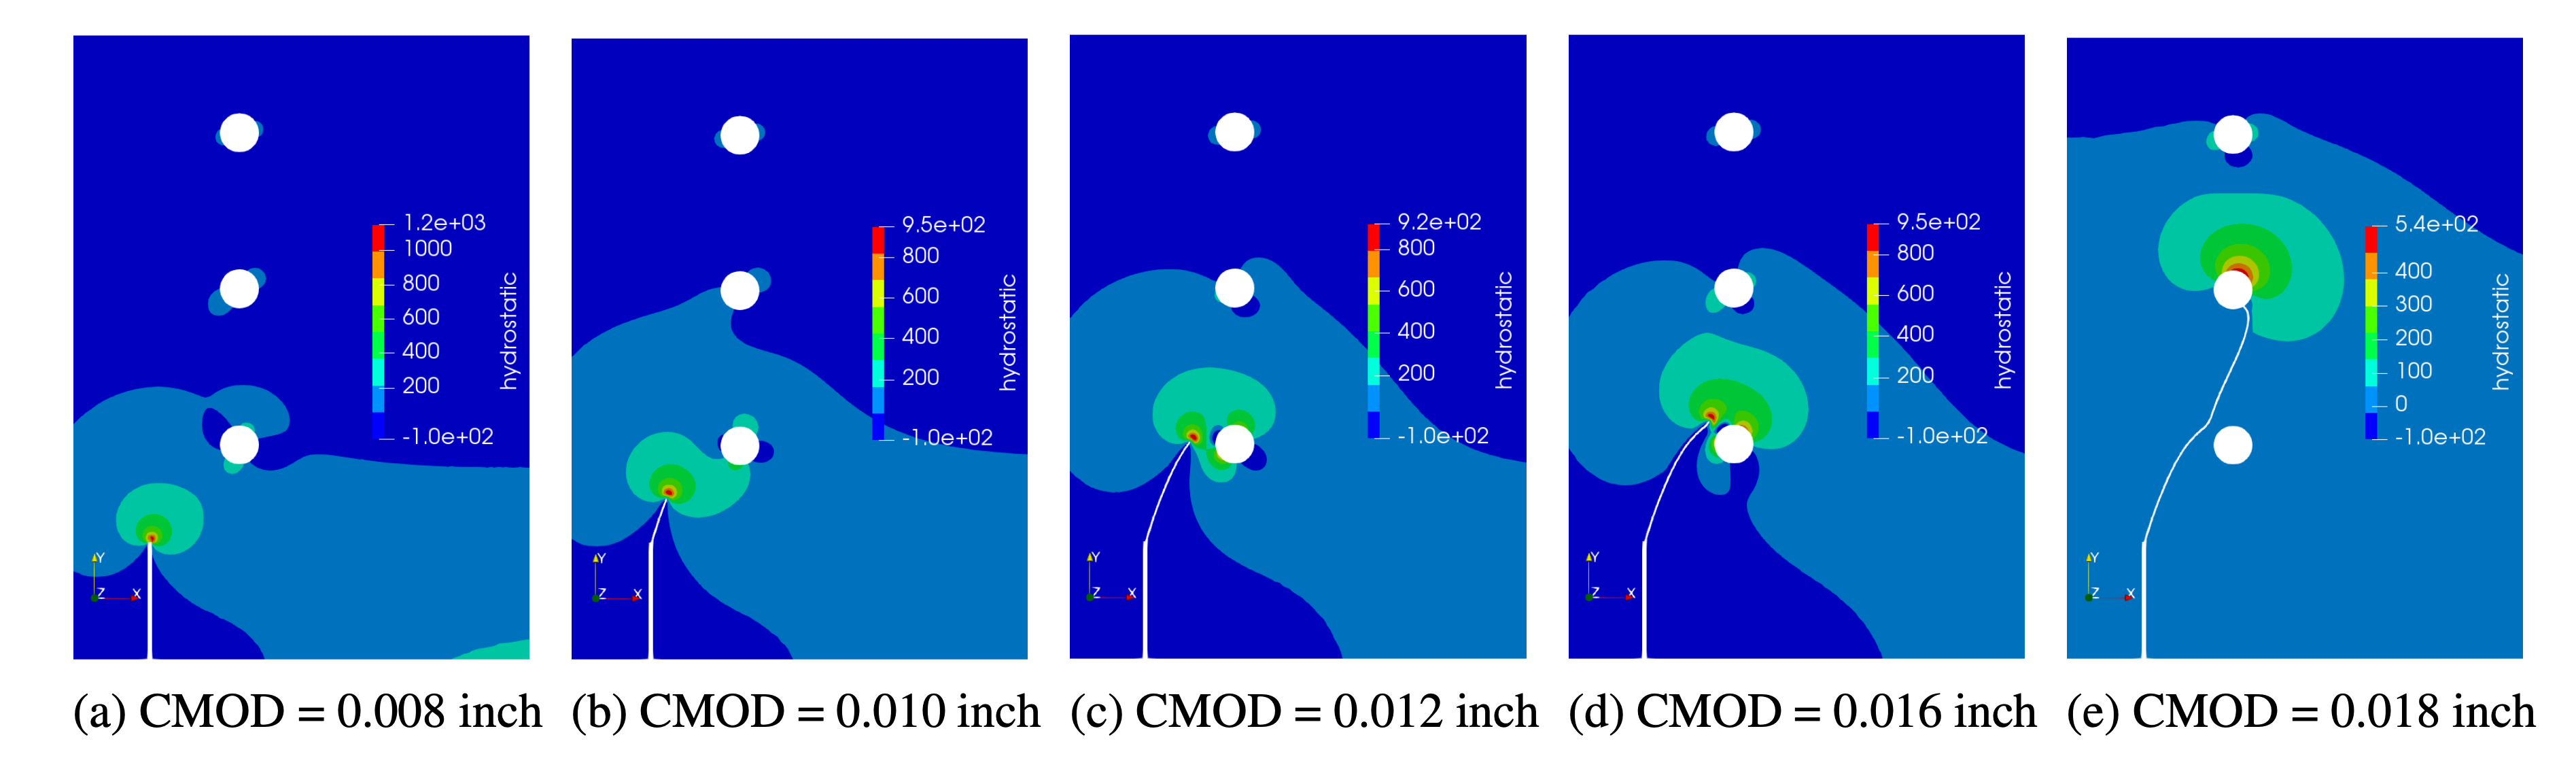
\includegraphics[width=0.9\textwidth]{figures1}
  \caption{A PGF figure of which the font matches the text font: 
  evolution of plastic strain $\varepsilon_p$ and temperature  $T$ in time.}
  \label{fig:figures1}
\end{figure}

%---------------------------------------------------------------------------
\begin{figure*}[!h]
  \begin{snippetlatex}[caption={Stacking multiple images using \LaTeX\ package \texttt{subfig}.},label={snippet_sub_figures},framerule=1pt,tabsize=3]
    \begin{figure}[h!] \centering
    \subfloat[CMOD=0.008 inch]{\includegraphics[width=0.18\textwidth]{t14} \label{fig:a}}\;
    \subfloat[CMOD=0.010 inch]{\includegraphics[width=0.18\textwidth]{t16} \label{fig:b}}\;
    \subfloat[CMOD=0.012 inch]{\includegraphics[width=0.18\textwidth]{t20} \label{fig:c}}\;
    \subfloat[CMOD=0.016 inch]{\includegraphics[width=0.18\textwidth]{t28} \label{fig:d}}\;
    \subfloat[CMOD=0.018 inch]{\includegraphics[width=0.18\textwidth]{t30} \label{fig:e}}\;
    \caption{Asymmetric notched beam under three-point bending: crack evolution.}
    \label{fig:bittencourt-evolution}
    \end{figure}
  \end{snippetlatex}
\end{figure*}
%---------------------------------------------------------------------------


\subsection{Tables}\label{sec:tabs}

Tables in scientific papers should be clear and focus on the data. We have found tables similar to \cref{table:params} satisfy all the criteria. The \LaTeX\ code is shown in \cref{snippet_latex_table}.


 \begin{table}[h!]
      \centering
      \caption{Material parameters and characteristics for all simulations.}
      \setlength\fboxsep{0pt}
      \vskip-\topsep%
      \smallskip%
      \renewcommand\arraystretch{1.4}
      \colorbox{darkgray}{%
      \begin{tabularx}{0.99\textwidth}{lllll}
      \toprule
      Parameter & Section 5.1 & Section 5.2 & Section 5.3 & Section 5.4 \\
      \midrule
        Young's modulus [MPa]     & $210\times10^3$ & 145 & 0.5887  & 6.5 \\
          Poisson's ratio [-]     & 0.3 & 0.45  & 0.45  & 0.45  \\
          Tensile strength [MPa]          & 2445  & 20  & 0.58 & 20  \\
          Fracture energy [N/mm]    & 2.7 & 2.4 & 2.67  & 15  \\
          Griffith's internal length [mm]     & 0.095 & 0.087 & 6.29  & 0.24 \\
          \midrule 
          Experimentally validated & n/a & n/a & yes & yes \\
          Solver & multi-step AM & single-step AM & implicit-explicit & implicit-explicit \\
          State & Plane strain & Plane strain & Plane strain & Plane stress \\
       \bottomrule
       \end{tabularx}%
      }
      \label{table:params}
      \end{table}


%---------------------------------------------------------------------------
\begin{figure*}[!h]
  \begin{snippetlatex}[caption={Typesetting tables in \LaTeX.},label={snippet_latex_table},framerule=1pt,tabsize=3]
      \begin{table}[h!]
      \centering
      \caption{Material parameters and characteristics for all simulations.}
      \setlength\fboxsep{0pt}
      \vskip-\topsep%
      \smallskip%
      \renewcommand\arraystretch{1.4}
      \colorbox{darkgray}{%
      \begin{tabularx}{0.99\textwidth}{lllll}
      \toprule
      Parameter & \cref{ex:brittle} & \cref{ex:penny} & \cref{ex:dens} & \cref{ex:mixed} \\
      \midrule
        Young's modulus [MPa]     & $210\times10^3$ & 145 & 0.5887  & 6.5 \\
          Poisson's ratio [-]     & 0.3 & 0.45  & 0.45  & 0.45  \\
          Tensile strength [MPa]          & 2445  & 20  & 0.58 & 20  \\
          Fracture energy [N/mm]    & 2.7 & 2.4 & 2.67  & 15  \\
          Griffith's internal length [mm]     & 0.095 & 0.087 & 6.29  & 0.24 \\
          \midrule 
          Experimentally validated & n/a & n/a & yes & yes \\
          Solver & multi-step AM & single-step AM & implicit-explicit & implicit-explicit \\
          State & Plane strain & Plane strain & Plane strain & Plane stress \\
       \bottomrule
       \end{tabularx}%
      }
      \label{table:params}
      \end{table}
  \end{snippetlatex}
\end{figure*}
%---------------------------------------------------------------------------


\subsection{Notations and equations}\label{sec:equation}

Avoid overly complex notations. Try to introduce a nomenclature in the paper, to ease things with the reviewers and readers.  Sometimes, a table such as the one \cref{tab:notations} does a good job to introduce main notations. 

%%%%%%%%%%%%%%%%%%%%%%%%%%%%%%%%%%%%%%%%%%%%%%%%%%
\setlength{\fboxsep}{0pt}
\begin{table}[h!]
   \centering
     \setlength\fboxsep{0pt}
\vskip-\topsep%
\smallskip%
%\renewcommand\arraystretch{1.3}
\colorbox{darkgray}{%
   \begin{tabularx}{0.6\textwidth}{llX}
   \toprule
   Variable & Type  & Meaning\\
  \midrule
  $\mathbf{x}_p$ & Vector & Particle position (time-dependent)\\
  $\mathbf{X}_p$ & Vector & Particle initial position\\
  $m_p$ & Scalar & Particle mass\\
  $V_p$ & Scalar & Particle volume\\
  $\rho_p$ & Scalar & Particle density\\
  $T_p$ & Scalar & Particle temperature\\
  $\mathbf{P}_p$ & Tensor/Matrix & Particle 1$^\text{st}$ Piola-Kirchoff stress\\
  \bottomrule
 \end{tabularx}%
 }
\caption{Major notations can be put in a table.}
 \label{tab:notations}
\end{table}
%%%%%%%%%%%%%%%%%%%%%%%%%%%%%%%%%%%%%%%%%%%%%%%%%%

%%%%%%%%%%%%%%%%%%%%%%%%%%%%%%%%%%%%%%%%%%%%%%%%%%
\setlength{\fboxsep}{0pt}
\begin{table}[h!]
   \centering
     \setlength\fboxsep{0pt}
\vskip-\topsep%
\smallskip%
%\renewcommand\arraystretch{1.3}
\colorbox{darkgray}{%
   \begin{tabularx}{0.7\textwidth}{ll}
   \toprule
   Don't & Do  \\
  \midrule
   $\varkappa$ & $\kappa$  \\
   $\hbar$ & $\bar{h}$  \\
   $\underline{\underline{A}}$ & $\boldsymbol{A}$ or $A_{ij}$\\
  \bottomrule
 \end{tabularx}%
 }
\caption{Avoid overly complex notations.}
 \label{tab:complex-notation}
\end{table}


%%%%%%%%%%%%%%%%%%%%%%%%%%%%%%%
\section{Submission}

With the pressure to “publish” (or perish), it is increasingly difficult for students to resist the temptation to submit a “large” number of papers during their PhD. Some supervisors will also push the students to publish “too many” papers. 

Do not submit until you are really happy with the work, as it usually does not save time to submit a piece of work which we know ourselves could be improved: the reviewers will think likewise, or be even more critical than we are ourselves of our work. If on a final read of the paper you think: “Ah… I could have added this study, this argument is not completely convincing to me, this graph could be better plotted, I think I forgot some relevant literature, the notations are complex, perhaps the reader will have difficulties…” then, do not submit, improve your work, and submit it when it is ready. 

It is also useful to ask peers to read over your work. Before giving your first draft to your supervisor(s), have it proof-read by a peer (if you are a PhD student, ask another PhD student for their opinion). This will bring the following positive points: 
It will value your peer as you think her/his opinion counts;
It will give you insights on how understandable your paper is by someone who is connected to your field but did not do exactly the same piece of research;
It will decrease the number of typos, which will enable your supervisor(s) to focus on the science as opposed to bumping over each spelling mistake, grammatical error, jargon.


%
%%%%%%%%%%%%%%%%%%%%%%%%%%%%%%%
\section*{Acknowledgments}

The first  author gratefully acknowledges the financial support of the Australian Research Council (ARC) Training Centre in Alloy Innovation for Mining Efficiency (IC160100036).
 The second author (V.P. Nguyen) thanks the funding support from the Australian Research Council via DECRA project DE160100577. 

%% The Appendices part is started with the command \appendix;
%% appendix sections are then done as normal sections
%=============================================================================
\begin{appendix}
%=============================================================================
%\showthe\textwidth % => width of the pdf, see in log file, is 468 pt. use it in plot.py for great plots.
\section{Python script for plotting data}

This appendix present some \texttt{Python} scripts to produce high quality plots which have the same font used in the paper. One can use the script shown in \cref{snippet_matplotlib} to get PDFs or the one in \cref{snippet_matplotlib_pgf} to get PGF files. PGF pictures can be embedded as raw commands in LaTeX documents.

The main idea is to get the correct figure size, and insert it in the paper without scaling. To determine the figure size, one first calculates the width of the paper, which can be done by inserting this command in the tex file:


\begin{verbatim}
\showthe\textwidth % => width of the pdf, see in log file, is 468 pt. 
\end{verbatim}
Then you can search for `width of the pdf' in this log file to find out the width of your paper.

\begin{figure*}[!h]
  \begin{snippet}[caption={Python script for plotting data.},label={snippet_matplotlib},framerule=1pt,tabsize=3]   
    import matplotlib as mpl
    import matplotlib.pyplot as plt

    def set_size(width, fraction=1, subplot=[1, 1]):
        if width == 'elsevier':
            width_pt = 468.
        elif width == 'beamer':
            width_pt = 307.28987
        else:
            width_pt = width
        fig_width_pt = width_pt * fraction      # Width of figure
        inches_per_pt = 1 / 72.27               # Convert from pt to inches
        golden_ratio = 0.75                     # (5**.5 - 1) / 2
        fig_width_in = fig_width_pt * inches_per_pt  # Figure width in inches
        fig_height_in = fig_width_in * golden_ratio * (subplot[0] / subplot[1])
        fig_dim = (fig_width_in, fig_height_in)
        return fig_dim

    parser = argparse.ArgumentParser(description='Plot the evolution of variables.',
                                     add_help=False,
                                     formatter_class=argparse.RawDescriptionHelpFormatter)


    parser.add_argument('--quiet', '-q', action='store_const', const=True, default=False,
                        help='do not show plot.')
    args = parser.parse_args()

    # Using seaborn's style
    plt.style.use('seaborn-colorblind')  

    nice_fonts = {
            "text.usetex": True,
            "font.family": "serif",
            "axes.labelsize": 10,
            "font.size": 10,
            "legend.fontsize": 8,
            "xtick.labelsize": 8,
            "ytick.labelsize": 8,
    }

    mpl.rcParams.update(nice_fonts)

    # Dimer 5: Read Data
    fnames = ['log.mpm', 'dam-break-Sun.csv', 'water-break-experiment.csv']
    dat    = [pylab.genfromtxt(f,skip_header=1) for f in fnames]

    fig, ax = plt.subplots(1, 1, figsize=set_size('elsevier', fraction=0.6))
    # fig, (ax1,ax2) = plt.subplots(1, 2, figsize=set_size(width, subplot=[1, 2]))

    for i, f in enumerate(fnames):   
        x = dat[i][:,3]
        y = dat[i][:,4]
        ax.plot(x, y, color='black', label='MPM',linewidth=1.5, linestyle='dotted')
       
        xmax = max(xmax, np.max(x))
        ymax = max(ymax, np.max(y))
         
    ax.set_xlabel(r'$T$')
    ax.set_ylabel(r'$L(T)$')
    ax.set_ylim(1.0, 2.8)
    ax.set_xlim(0, 1.6)
    ax.legend(loc=0)
    plt.tight_layout()
    plt.savefig('./water-break-plot.pdf', format='pdf', bbox_inches='tight')

    if args.quiet == False:
        plt.show()
  \end{snippet}
\end{figure*}

\begin{figure*}[!h]
  \begin{snippet}[caption={Python script for plotting data.},label={snippet_matplotlib_pgf},framerule=1pt,tabsize=3]   
    nice_fonts = {
            "text.usetex": True,
            "font.family": "serif",
            "pgf.texsystem": "pdflatex",
            "font.family": "serif",
            "font.serif": [],
            "font.sans-serif": [],
            "font.monospace": [],
            "pgf.preamble": [
            # put LaTeX preamble declarations here
            r"\usepackage[utf8x]{inputenc}",
            r"\usepackage[T1]{fontenc}",
            # macros defined here will be available in plots, e.g.:
            r"\newcommand{\vect}[1]{#1}",
            # You can use dummy implementations, since you LaTeX document
            # will render these properly, anyway.
            ],
            "axes.labelsize": 10,
            "font.size": 10,
            "legend.fontsize": 8,
            "xtick.labelsize": 8,
            "ytick.labelsize": 8,
    }
    plt.savefig('./cold-spray-plots.pgf', bbox_inches='tight') 
    if args.quiet == False:
        plt.show()
  \end{snippet}
\end{figure*}


\end{appendix}


%%%%%%%%%%%%%%%%%%%%%%%%
%\section*{References}


% %%%%%%% BIB files (bibtex)
%\bibliographystyle{plainnat}
\bibliographystyle{abbrvnat} % => just V. P. Nguyen, not Phu Nguyen, ...
%\bibliographystyle{natbib}
\bibliography{writing}

% if biblatex is used
%\printbibliography

\end{document}
